\renewcommand{\thislecture}{1 }

%
% Cover page
%

\title[Neutrino Physics / Lecture \thislecture]
{
  {\huge \color{yellow} Neutrino Physics - Lecture \thislecture} \\
  {\it Neutrino Oscillation Phenomenology}\\
}

\author[C.Andreopoulos] {
  Professor Costas Andreopoulos\inst{1,2}
}
\institute[Liverpool/STFC-RAL] {
   \inst{1} University of Liverpool,
   \inst{2} STFC Rutherford Appleton Laboratory\\
   \vspace{0.5cm}
   {\it {\color{magenta} A post-graduate student lecture course}}\\
   \vspace{0.2cm}
}
\date{\today}

\titlegraphic{
  
\includegraphics[height=25px]{./images/logo/liverpool.png}
  \hspace{3px}
  
\includegraphics[height=30px]{./images/logo/ral.png}
}

	



\begin{frame}[plain]
  \titlepage
\end{frame}

%
% Outline
%

\begin{frame}{Outline for Lecture \thislecture}

\begin{itemize}
  \item Neutrino oscillations
  \item Neutrino oscillation probability calculation in vacuum
  \item Two-flavour and three-flavour case
  \item Types of oscillation measurements
  \item The exclusion plot
  \item Neutrino oscillation probability calculation in matter
  \item MSW effect
  \item Antineutrino oscillation probabilities
  \item Interdependencies of oscillation channels
  \item Effect of T, CP and CPT symmetries of neutrino oscillations
  \item The big picture - current knowledge
\end{itemize}

\end{frame}

%
%
%

% \begin{frame}{Neutrino oscillations}
%
% {\scriptsize
% \begin{columns}[T]
%  \begin{column}{0.40\textwidth}
%   \begin{block}{}
%   {\bf Production \& Detection} \\
%   \vspace{0.1cm}
%   Flavour eigenstates\\
%     \hspace{0.3cm} - $\nu_{e}$, $\nu_{\mu}$, $\nu_{\tau}$, ...\\
%   Interactions described by:\\
%     \hspace{0.3cm} $\mathcal{L}_{CC}=\frac{g}{2\sqrt{2}} j_{CC}^{\mu} W_{\mu} + h.c.$\\
%   \end{block}
%   \begin{block}{}
%   {\bf Propagation} \\
%   \vspace{0.1cm}
%   Mass eigenstates:\\
%      \hspace{0.3cm} - $\nu_{1}$, $\nu_{2}$, $\nu_{3}$, ...\\
%   Described by plane waves:\\
%      \hspace{0.3cm} $|\nu_{i}(L)>=e^{-im_{i}^{2}L/2E}{\cdot}|\nu_{i}(0)>$\\
%   \end{block}
%   \begin{block}{}
%   Each flavour eigenstate a superposition of mass eigenstates
%   \begin{equation}
%    \nonumber
%    \begin{pmatrix}
%     \nu_{e}\\ \nu_{\mu}\\ \nu_{\tau}
%    \end{pmatrix}
%    =
%    \begin{pmatrix}
%      U_{e1} & U_{e2} & U_{e3} \\
%      U_{\mu1} & U_{\mu2} & U_{\mu3} \\
%      U_{\tau1} & U_{\tau2} & U_{\tau3} \\
%    \end{pmatrix}
%    \begin{pmatrix}
%     \nu_{1}\\ \nu_{2}\\ \nu_{3}
%    \end{pmatrix}
%   \end{equation}
%   \end{block}
%
%  \end{column}
%  \begin{column}{0.60\textwidth}
%    \begin{center}
%    {\bf A quantum-mechanical interference effect}\\
%    \vspace{0.3cm}
%    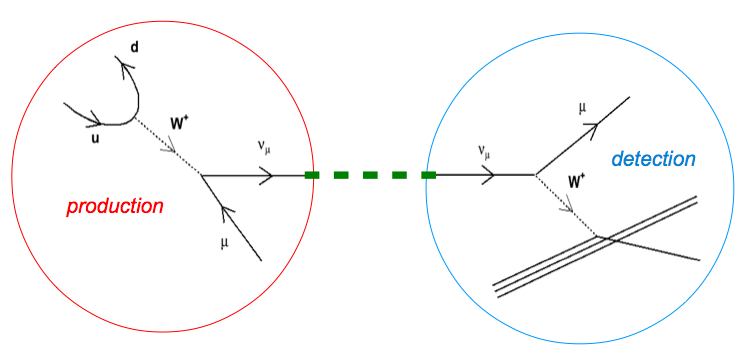
\includegraphics[width=0.95\textwidth]{./images/osc101/osc_schematic.png}\\
%    \vspace{0.3cm}
%    A neutrino state that starts its life as particular flavour eigenstate (e.g. $\nu_{\mu}$)
%    may be detected as a different flavour eigenstate (e.g. $\nu_{e}$).\\
%    \end{center}
%  \end{column}
% \end{columns}
% }
% \end{frame}


%
%
%

\begin{frame}{Neutrino oscillations}

   \begin{center}
   {\bf Neutrino oscillations is a quantum-mechanical interference effect}\\
   \vspace{0.3cm}
   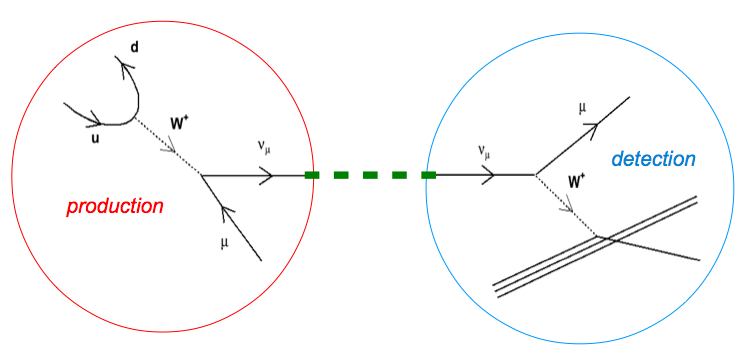
\includegraphics[width=0.95\textwidth]{./images/osc101/osc_schematic.png}\\
   \vspace{0.3cm}
   A neutrino state that starts its life as particular flavour eigenstate\\ (e.g. $\nu_{\mu}$)
   may be detected as a different flavour eigenstate (e.g. $\nu_{e}$).\\
   \end{center}

\end{frame}


%
%
%

\begin{frame}{Neutrino oscillations}

\begin{columns}
 \begin{column}{0.50\textwidth}
  Each flavour eigenstate is a {\bf superposition of mass eigenstates}.
  \begin{equation}
   \nonumber
   \begin{pmatrix}
    \nu_{e}\\ \nu_{\mu}\\ \nu_{\tau}
   \end{pmatrix}
   =
   \underbrace{
   \begin{pmatrix}
     U_{e1} & U_{e2} & U_{e3} \\
     U_{\mu1} & U_{\mu2} & U_{\mu3} \\
     U_{\tau1} & U_{\tau2} & U_{\tau3} \\
   \end{pmatrix}
   }_\text{$U_{PMNS}$}
   \begin{pmatrix}
    \nu_{1}\\ \nu_{2}\\ \nu_{3}
   \end{pmatrix}
  \end{equation}\\
  \vspace{0.3cm}
   For antineutrinos:
  \begin{equation}
   \nonumber
   U_{PMNS} \rightarrow U^{\star}_{PMNS}
  \end{equation}\\
  {\scriptsize \color{magenta} {\bf PMNS}: {\bf P}ontecorvo-{\bf M}aki-{\bf
      N}akagawa-{\bf S}akata}
 \end{column}
 \begin{column}{0.50\textwidth}
   \begin{center}
   \vspace{0.3cm}
   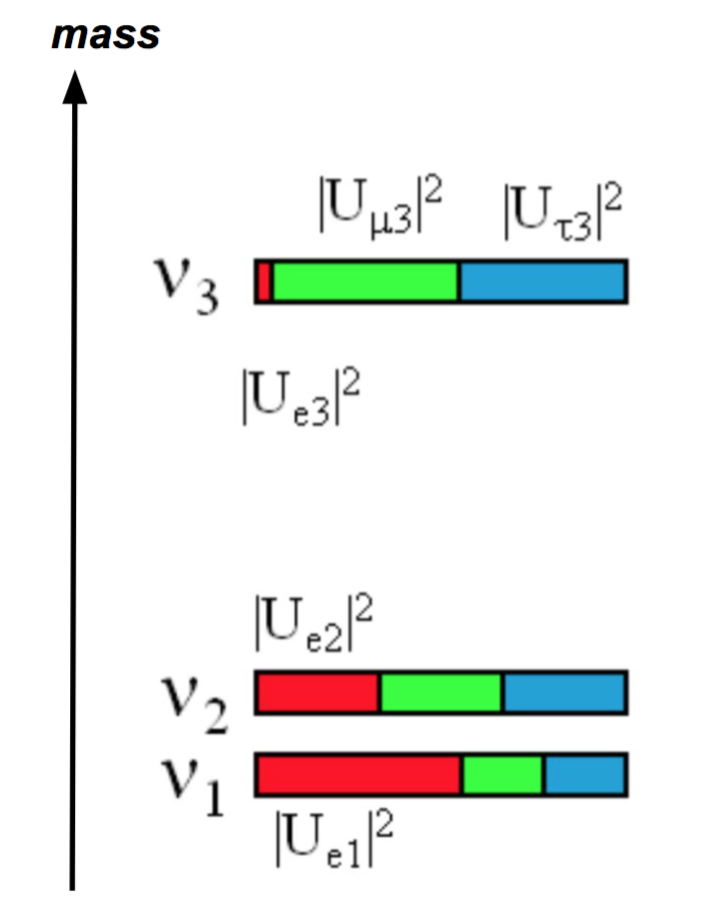
\includegraphics[width=0.80\textwidth]{./images/osc101/mass_spectrum_01}\\
   \vspace{0.3cm}
   \end{center}
 \end{column}
\end{columns}

\end{frame}


%
%
%

\begin{frame}{Neutrino oscillations}

\begin{center}
   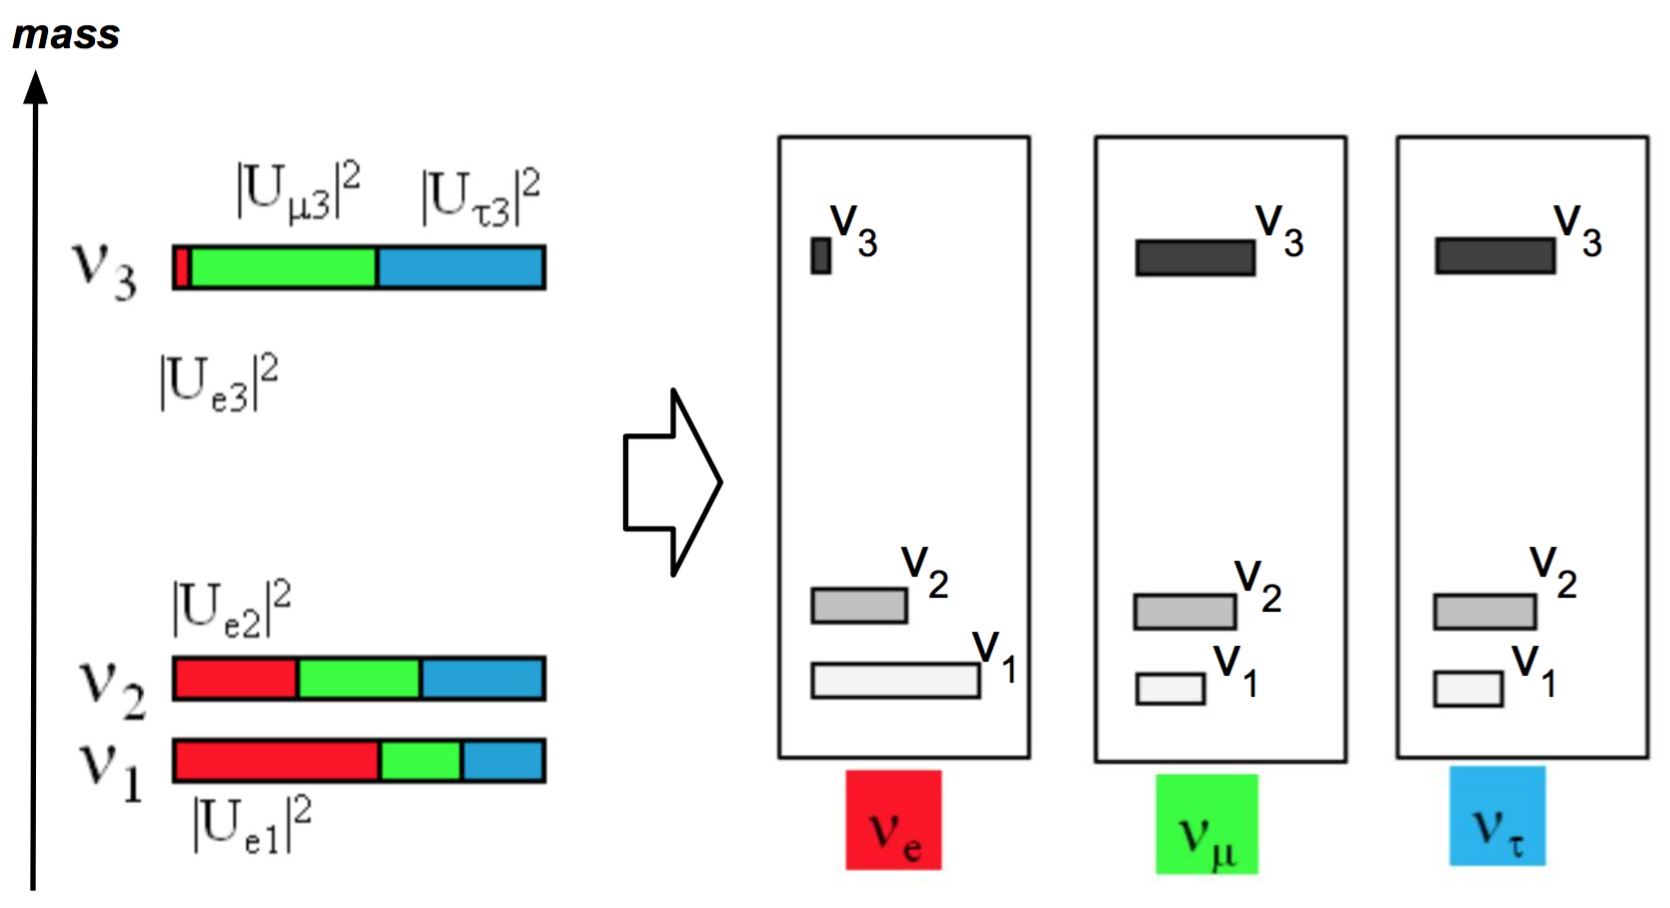
\includegraphics[width=0.95\textwidth]{./images/osc101/mass_spectrum_2_flavours_01}\\
\end{center}

\end{frame}

%
%
%

\begin{frame}{Neutrino oscillations}

\begin{columns}
 \begin{column}{0.30\textwidth}
   \begin{center}
   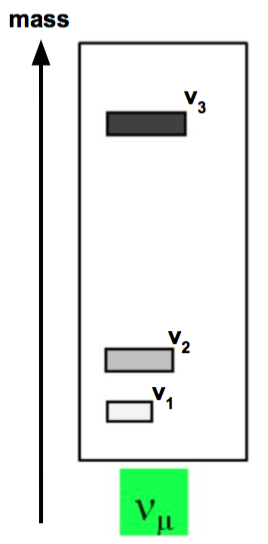
\includegraphics[width=0.90\textwidth]{./images/osc101/mass_spectrum_numu_02}\\
   \end{center}
 \end{column}
 \begin{column}{0.70\textwidth}
   A muon-neutrino,
   {\bf at the very moment it gets created}, is described by the
   following state:
   \begin{equation}
     \nonumber
       |\nu_{\mu}> \; \approx \;
              {\color{magenta}0.4} \cdot |\nu_1> + \;
              {\color{magenta} 0.6} \cdot |\nu_2> +
              {\color{magenta} 0.7} \cdot |\nu_3>
   \end{equation}
   \begin{center}
     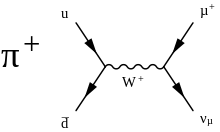
\includegraphics[width=0.35\textwidth]{./images/osc101/piplus_muon_decay}\\
   \end{center}
   So, at that time, a muon-neutrino is:
   \begin{itemize}
           \item $100 * ({\color{magenta}0.4})^2 \approx {\color{magenta}15\%} \; \nu_{1}$
           \item $100 * ({\color{magenta}0.6})^2 \approx {\color{magenta}35\%} \; \nu_{2}$
           \item $100 * ({\color{magenta}0.7})^2 \approx {\color{magenta}50\%} \; \nu_{3}$
   \end{itemize}
 \end{column}
\end{columns}

\end{frame}

%
%
%

\begin{frame}{Neutrino oscillations}

\begin{columns}
 \begin{column}{0.60\textwidth}
   \begin{center}
   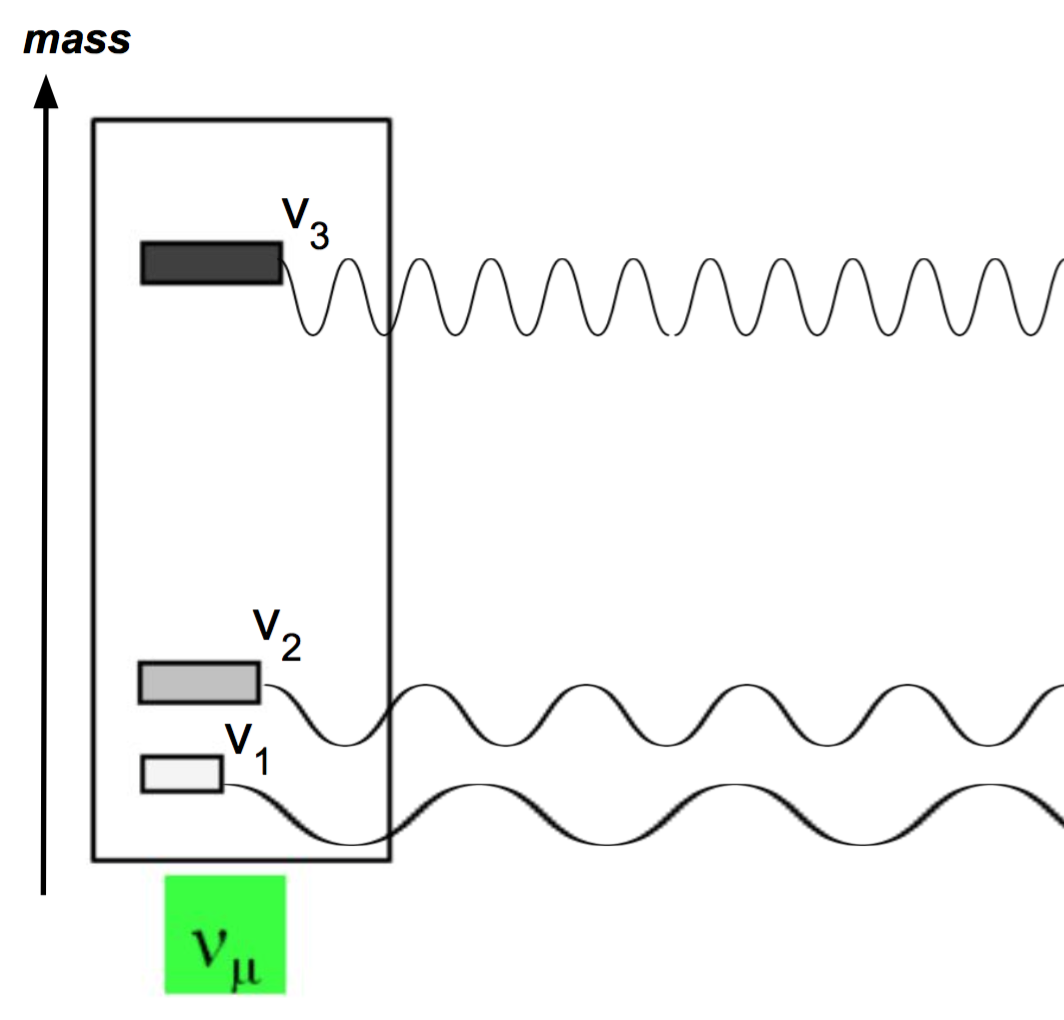
\includegraphics[width=0.88\textwidth]{./images/osc101/numu_propagation_01}\\
   \end{center}
 \end{column}
 \begin{column}{0.40\textwidth}
  The propagation of each mass eigenstate i (i=1,2,3)\\ is described by a plane wave:\\
     \hspace{0.3cm} $|\nu_{i}(L)>=e^{-i {\bf
         \color{magenta}m_{i}^{2}}L/2E}{\cdot}|\nu_{i}(0)>$\\
  \vspace{0.4cm}
  Immediately after its creation, {\bf the superposition} that makes up a
  flavour eigenstate {\bf gets altered}.\\
  \vspace{0.2cm}
  The neutrino now has a {\bf finite probability to be observed as a
  different flavour state}.
 \end{column}
\end{columns}

\end{frame}

%
%
%

{

\setbeamercolor {frametitle}          {bg=dBG1}
\setbeamercolor {author in head/foot} {bg=dBG1}
\setbeamercolor {title in head/foot}  {bg=dBG2}
\setbeamercolor {date in head/foot}   {bg=dBG3}
\setbeamercolor {date in head/foot}   {fg=dFG3}

%
%
%

\begin{frame}{Neutrino oscillation probability calculation in vacuum}

A flavour eigenstate $|\nu_{\beta}>$ can be written as a linear superposition
of mass eigenstates $|\nu_{k}>$
\begin{equation*}
    |\nu_{\beta}> = \sum_{k} U_{{\beta}k} |\nu_{k}>
\end{equation*}

The $|\nu_{k}>$ states propagate according to the time-dependent Schrodinger equation
\begin{equation*}
    i \frac{\partial}{\partial t} |\nu_{k}(x,t)> = E |\nu_{k}(x,t)>
     = - \frac{1}{2m_{k}} \frac{\partial^{2}}{\partial x^{2}} |\nu_{k}(x,t)>
\end{equation*}

The solution to this equation is a plane wave
\begin{equation*}
    |\nu_{k}(x,t)> = e^{-i(E_{k}t-p_{k}x)} |\nu_{k}(0,0)>
\end{equation*}

\end{frame}

%
%
%

\begin{frame}{Neutrino oscillation probability calculation in vacuum}

Therefore, at (x,t), the flavour eigenstate $|\nu_{\beta}>$ can be written as
\begin{equation*}
    |\nu_{\beta}(x,t)> = \sum_{k} U_{{\beta}k} |\nu_{k}(x,t)> \Rightarrow
\end{equation*}
\begin{equation*}
    |\nu_{\beta}(x,t)> = \sum_{k} U_{{\beta}k} e^{-i(E_{k}t-p_{k}x)} |\nu_{k}(0,0)>
\end{equation*}

Inverting the mixing matrix, we can write
\begin{equation*}
    |\nu_{k}(0,0)> = \sum_{\gamma} U^{\star}_{{\gamma}k} |\nu_{\gamma}(0,0)>
\end{equation*}

Therefore
\begin{equation*}
    |\nu_{\beta}(x,t)> =
       \sum_{k} U_{{\beta}k} e^{-i(E_{k}t-p_{k}x)}
       \sum_{\gamma} U^{\star}_{{\gamma}k} |\nu_{\gamma}(0,0)> \Rightarrow
\end{equation*}
\begin{equation*}
    |\nu_{\beta}(x,t)> =
        \sum_{\gamma} \sum_{k}
          U^{\star}_{{\gamma}k} e^{-i(E_{k}t-p_{k}x)} U_{{\beta}k}
          |\nu_{\gamma}(0,0)>
\end{equation*}

\end{frame}

%
%
%

\begin{frame}{Neutrino oscillation probability calculation in vacuum}

The transition amplitude for detecting a neutrino of flavour $\beta$ at (x,t),
given that it was produced as flavour $\alpha$ at (0,0) is

\begin{equation*}
   A_{\alpha \beta} = <\nu_{\beta}(x,t)|\nu_{\alpha}(0,0)> \Rightarrow
\end{equation*}
\begin{equation*}
   A_{\alpha \beta} =
     \sum_{\gamma} \sum_{k}
     U_{{\gamma}k} e^{i(E_{k}t-p_{k}x)} U^{\star}_{{\beta}k}
     \cancelto{\delta_{\gamma \alpha}}{<\nu_{\gamma}(0,0)|\nu_{\alpha}(0,0)>} \Rightarrow
\end{equation*}
\begin{equation*}
   A_{\alpha \beta} =
     \sum_{k}
     U_{{\alpha}k} e^{i(E_{k}t-p_{k}x)} U^{\star}_{{\beta}k}
\end{equation*}

The oscillation probability is given by
\begin{equation*}
   P_{\alpha \beta} = |A_{\alpha \beta}|^2 =
     |\sum_{k} U_{{\alpha}k} e^{i(E_{k}t-p_{k}x)} U^{\star}_{{\beta}k}|^2 \Rightarrow
\end{equation*}
% \begin{equation*}
%      P_{\alpha \beta} =
%         \sum_{k} U_{{\alpha}k} e^{i(E_{k}t-p_{k}x)} U^{\star}_{{\beta}k}
%         \sum_{\ell} U^{\star}_{{\alpha}\ell} e^{-i(E_{\ell}t-p_{\ell}x)} U_{{\beta}\ell}
%      \Rightarrow
% \end{equation*}
\begin{equation*}
     P_{\alpha \beta} =
        \sum_{k} \sum_{\ell}
        U_{{\alpha}k} U^{\star}_{{\beta}k}
        U^{\star}_{{\alpha}\ell} U_{{\beta}\ell}
        e^{i( (E_{k}-E_{\ell})t-(p_{k}-p_{\ell})x)}
\end{equation*}

\end{frame}

%
%
%

\begin{frame}{Two-flavour oscillation probability calculation in vacuum}

  Since neutrinos are relativistic, $t \approx x = L$ (c = 1),
  where L is the distance between the source and the detector.
  In this case
  \begin{equation*}
    (E_{k}-E_{\ell})t-(p_{k}-p_{\ell})x \approx \frac{\Delta m^{2}_{k \ell}}{2E}L
  \end{equation*}
  where $\Delta m^{2}_{k \ell} = m^{2}_{k}-m^{2}_{\ell}$.\\
  \vspace{0.3cm}
  Therefore, the oscillation probability can be written as
  \begin{equation*}
  {\color{magenta}
   P_{\alpha \beta} =
      \sum_{k} \sum_{\ell}
      U_{{\alpha}k} U^{\star}_{{\beta}k}
      U^{\star}_{{\alpha}\ell} U_{{\beta}\ell}
      e^{i \frac{\Delta m^{2}_{k \ell}}{2E}L}
  }
  \end{equation*}

  \noindent\rule{2cm}{0.4pt}\\
  {
  \scriptsize
  \begin{equation*}
    (E_{k}-E_{\ell})t-(p_{k}-p_{\ell})x =
    \Big\{E_{k}-E_{\ell}-p_{k}+p_{\ell}\Big\}L =
  \end{equation*}
  \begin{equation*}
    \Big\{E_{k}-E_{\ell}-\sqrt{E^{2}_{k}-m^{2}_{k}}+\sqrt{E^{2}_{\ell}-m^{2}_{\ell}}\Big\}L =
    \Big\{E_{k}-E_{\ell}-
         E_{k}    \sqrt{1-\frac{m^{2}_{k}}   {E^{2}_{k}}} +
         E_{\ell} \sqrt{1-\frac{m^{2}_{\ell}}{E^{2}_{\ell}}})\Big\}L \approx
  \end{equation*}
  \begin{equation*}
    \Big\{E_{k}-E_{\ell}-
         E_{k}    (1-\frac{m^{2}_{k}}   {2E^{2}_{k}})+
         E_{\ell} (1-\frac{m^{2}_{\ell}}{2E^{2}_{\ell}}) \Big\}L =
    \Big\{E_{k} - E_{\ell} -
          E_{k}    + \frac{m^{2}_{k}}   {2E_{k}} +
          E_{\ell} - \frac{m^{2}_{\ell}}{2E_{\ell}} \Big\}L \approx \frac{\Delta m^{2}}{2E}L
  \end{equation*}
  }

\end{frame}


%
%
%

\begin{frame}{Two-flavour oscillation probability calculation in vacuum}

We can easily evaluate the terms
\begin{equation*}
  c_{\alpha \beta; k \ell} =
   U_{{\alpha}k} U^{\star}_{{\beta}k}
   U^{\star}_{{\alpha}\ell} U_{{\beta}\ell}
   e^{i \frac{\Delta m^{2}_{k \ell}}{2E}L}
\end{equation*}

in a framework with two flavours ($\alpha$, $\beta$), where
\begin{equation}
 \nonumber
 \begin{pmatrix}
  \nu_{\alpha}\\ \nu_{\beta}
 \end{pmatrix}
 =
 \begin{pmatrix}
   cos\theta & sin\theta \\
  -sin\theta & cos\theta \\
 \end{pmatrix}
 \begin{pmatrix}
  \nu_{1}\\ \nu_{2}
 \end{pmatrix}
\end{equation}

We find
\begin{itemize}
\small
  \item
  $c_{\alpha \beta; 11}$ =
  $U_{{\alpha}1} U^{\star}_{{\beta}1}
   U^{\star}_{{\alpha}1} U_{{\beta}1}
   e^{i \frac{\Delta m^{2}_{11}}{2E}L} =
   |U_{{\alpha}1}|^2 |U_{{\beta}1}|^2$ =
   $cos^2\theta sin^2\theta$
  \item
  $c_{\alpha \beta; 12}$ =
  $U_{{\alpha}1} U^{\star}_{{\beta}1}
  U^{\star}_{{\alpha}2} U_{{\beta}2}
  e^{i \frac{\Delta m^{2}_{12}}{2E}L}$ =
  $- cos^2\theta sin^2\theta
  e^{-i \frac{\Delta m^{2}_{21}}{2E}L}$
  \item
  $c_{\alpha \beta; 21}$ =
  $U_{{\alpha}2} U^{\star}_{{\beta}2}
  U^{\star}_{{\alpha}1} U_{{\beta}1}
  e^{i \frac{\Delta m^{2}_{21}}{2E}L}$ =
  $- cos^2\theta sin^2\theta
  e^{i \frac{\Delta m^{2}_{21}}{2E}L}$
  \item
  $c_{\alpha \beta; 22}$ =
  $U_{{\alpha}2} U^{\star}_{{\beta}2}
  U^{\star}_{{\alpha}2} U_{{\beta}2}
  e^{i \frac{\Delta m^{2}_{22}}{2E}L}$ =
  $|U_{{\alpha}2}|^2 |U_{{\beta}2}|^2$ =
  $cos^2\theta sin^2\theta$
\end{itemize}

\end{frame}

%
%
%

\begin{frame}{Two-flavour oscillation probability calculation in vacuum}

Therefore, the two-flavour oscillation probability can be written as

\begin{equation*}
     P_{\alpha \beta} =
      2 cos^2\theta sin^2\theta -
      cos^2\theta sin^2\theta
      (e^{-i \frac{\Delta m^{2}_{21}}{2E}L} +
       e^{ i \frac{\Delta m^{2}_{21}}{2E}L})
     \Rightarrow
\end{equation*}

\begin{equation*}
     P_{\alpha \beta} =
      2 cos^2\theta sin^2\theta -
      2 cos^2\theta sin^2\theta cos\Big(\frac{\Delta m^{2}_{21}}{2E}L\Big)
     \Rightarrow
\end{equation*}

\begin{equation*}
     P_{\alpha \beta} =
      2 cos^2\theta sin^2\theta \Big\{1 - cos\Big(\frac{\Delta m^{2}_{21}}{2E}L\Big)\Big\}
     \Rightarrow
\end{equation*}


Remembering that $cos\theta sin\theta = \frac{1}{2}sin(2\theta)$ and
$1-cos(2\theta)=2sin^{2}(\theta)$, the above expression for $P_{\alpha \beta}$ becomes

\begin{equation*}
{\color{magenta}
  P_{\alpha \beta} = sin^{2} (2\theta) sin^2\Big(\frac{\Delta m^{2}_{21}}{4E}L\Big)
}
\end{equation*}

\end{frame}


%
%
%

\begin{frame}{Two-flavour neutrino oscillation probability}

  The two-flavour oscillation formula derived previously
  \begin{equation*}
       P_{\alpha \beta} = sin^{2} (2\theta) sin^2(\frac{\Delta m^{2}_{21}L}{4E})
  \end{equation*}

  is often written as
  \begin{equation*}
       P_{\alpha \beta} = sin^{2} (2\theta) sin^2(1.27 \frac{\Delta m^{2}_{21}L}{E})
  \end{equation*}

  \vspace{0.3cm}

  Here, the 1.27 is a {\bf dimensional factor} allowing one to express
  \begin{itemize}
    \item $\Delta m^{2}_{21}$ in $eV^{2}$
    \item L/E in km/GeV or m/MeV
  \end{itemize}
\end{frame}

} % color

%
%
%
\begin{frame}{Two-flavour neutrino oscillation probability}

  The two-flavour oscillation formula can be written as
  \begin{equation*}
       P_{\alpha \beta} = sin^{2} (2\theta) sin^2(1.27 \frac{\Delta m^{2}L}{E})
  \end{equation*}

  \vspace{0.3cm}
  Despite the obvious limitation (two-flavours) the above expression is a sufficient approximation
  when, as it often happens, oscillation effects from a single $\Delta m^{2}$ scale dominate.\\

  \vspace{0.2cm}
  \begin{block}{}
  {\scriptsize
    It is worth remembering the assumptions under which this was derived:
    \begin{itemize}
    \item neutrino flavour and mass states are mixed, and
    \item we create a {\bf coherent superposition} of mass states at the weak interaction vertex
    \end{itemize}
    \vspace{0.3cm}
    {\bf Question}: \\
    What would happen if we did know which mass state was created at the vertex?
  }
  \end{block}

\end{frame}


\begin{frame}{Two-flavour neutrino oscillation probability}

{\bf Question}: \\
What would happen if we did know which mass state was created at the vertex?\\
\vspace{0.3cm}

\begin{itemize}
  \item There would be {\bf no flavour oscillation}
  \begin{itemize}
    \item No superposition $\rightarrow$ no phase difference
  \end{itemize}
  \item But there would be {\bf flavour change}
  \begin{itemize}
    \item Suppose we produce a lepton flavour $\alpha$ and mass state $|\nu_k>$
    \begin{itemize}
      \item The probability for the above is $|<\nu_k|\nu_{\alpha}>|^2=|U_{k\alpha}|^2$
    \end{itemize}
    \item This mass state propagates and can be detected as a state of flavour $\beta$
    \begin{itemize}
      \item The probability for the above is $|<\nu_{\beta}|\nu_{k}>|^2=|U_{\beta k}|^2$
    \end{itemize}
    \item Therefore the probability for flavour change is
    \begin{equation*}
         P_{\alpha \beta} = \sum_k |U_{\beta k}|^2 |U_{k\alpha}|^2
    \end{equation*}
    \item In the 2-flavor case, the above becomes
    \begin{equation*}
         P_{\alpha \beta} =
         |U_{\alpha 1}|^2 |U_{\beta 1}|^2 + |U_{\alpha 2}|^2 |U_{\beta 2}|^2 =
         2 cos^2\theta sin^2\theta = \frac{1}{2} sin^2(2\theta)
    \end{equation*}

  \end{itemize}

\end{itemize}

\end{frame}

%
%
%

\begin{frame}{Two-flavour neutrino oscillation probability}

  \begin{center}
    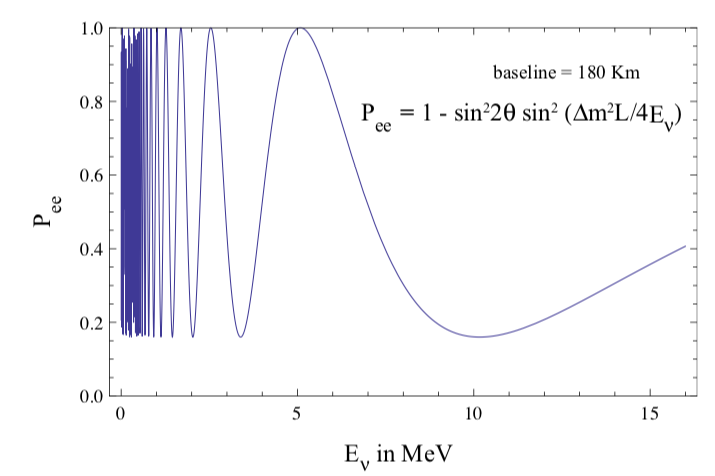
\includegraphics[width=0.75\textwidth]{./images/osc101/Pee_2flavour_pdg}\\
    \vspace{0.4cm}
    $\nu_{e}$ survival probability as function of the neutrino energy for L = 180 km,
    $\Delta m^{2}$ = 7$\times$10$^{-5}$ eV$^{2}$ and sin$^2$2$\theta$ = 0.84.
  \end{center}

\end{frame}

%
%
%

\begin{frame}{Signatures of neutrino mixing}

  \begin{center}
    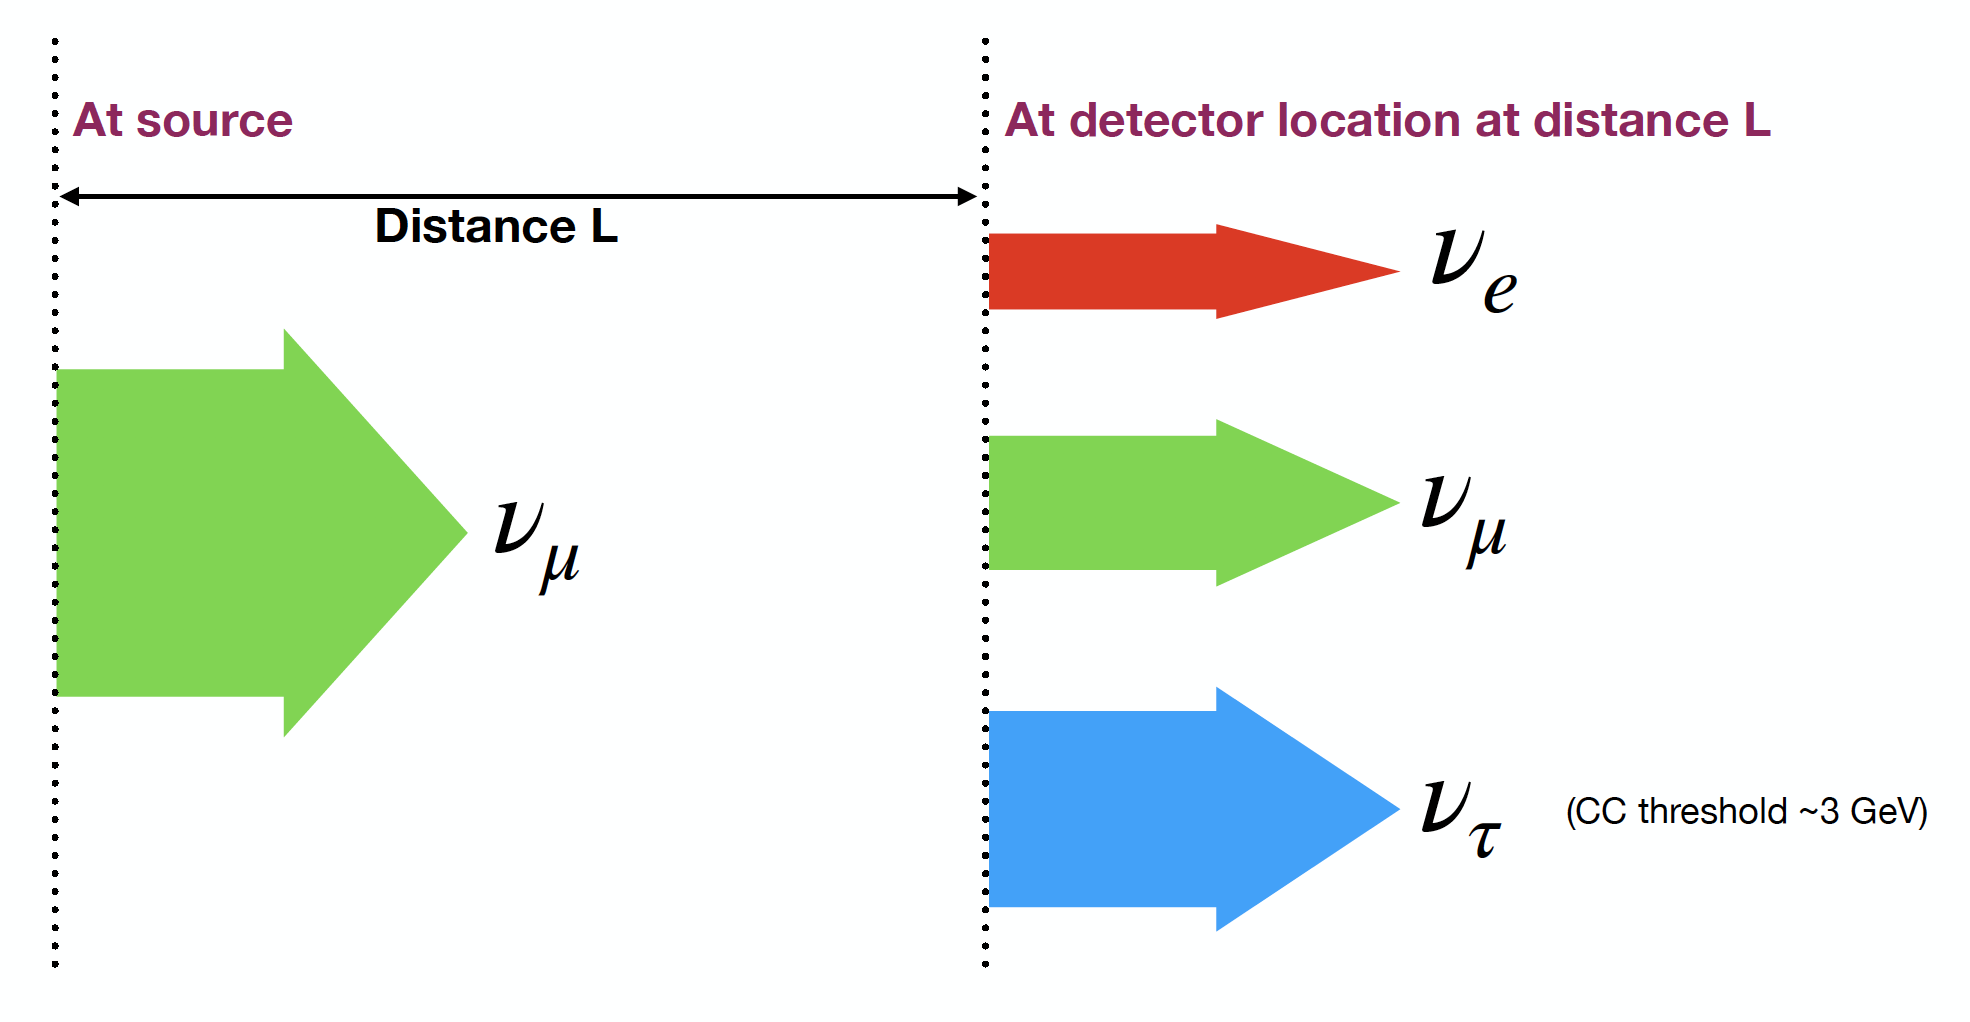
\includegraphics[width=0.95\textwidth]{./images/osc101/oscillation_signatures}\\
    \vspace{0.4cm}
    Neutrino {\bf \color{blue} disappearance} and neutrino {\bf \color{red} appearance}.
  \end{center}

\end{frame}

%
%
%

\begin{frame}{Two types of oscillation measurements}

There are two types of measurements one could try and do:

\begin{itemize}

  \item Measure {\bf neutrino disappearance}:
   Start with a neutrino beam of flavor $\alpha$ and determine the neutrino survival probability.
  \begin{equation*}
       P_{\alpha \alpha} = 1 - P_{\alpha \beta} =
       1 - sin^{2} (2{\color{red}\theta}) sin^2(1.27 \frac{{\color{red}\Delta m^{2}}L}{E})
  \end{equation*}

  \item Measure {\bf neutrino appearance}:
  Start with a neutrino beam of flavor $\alpha$ and try to establish the presence
  of neutrinos of flavour $\beta$.
  \begin{equation*}
       P_{\alpha \beta} = sin^{2} (2{\color{red}\theta}) sin^2(1.27 \frac{{\color{red}\Delta m^{2}}L}{E})
  \end{equation*}

\end{itemize}

In both cases, the objective is to determine the {\bf mixing parameter {\color{red} $\theta$}}
and the {\bf squared mass splitting {\color{red}$\Delta m^{2}$}}.\\
\vspace{0.2cm}
The ratio of $L/E$ is tuned to explore the {\color{red}($\theta$, $\Delta m^{2}$)} space.\\

\noindent\rule{2cm}{0.4pt}\\
{
\tiny
Neutrino energy is almost always a distribution,
in which case one tries to match $L/E_{peak}$ to the
squared mass splitting region to be investigated.\\
}

\end{frame}

%
%
%

\begin{frame}{Neutrino disappearance}

  \begin{center}
    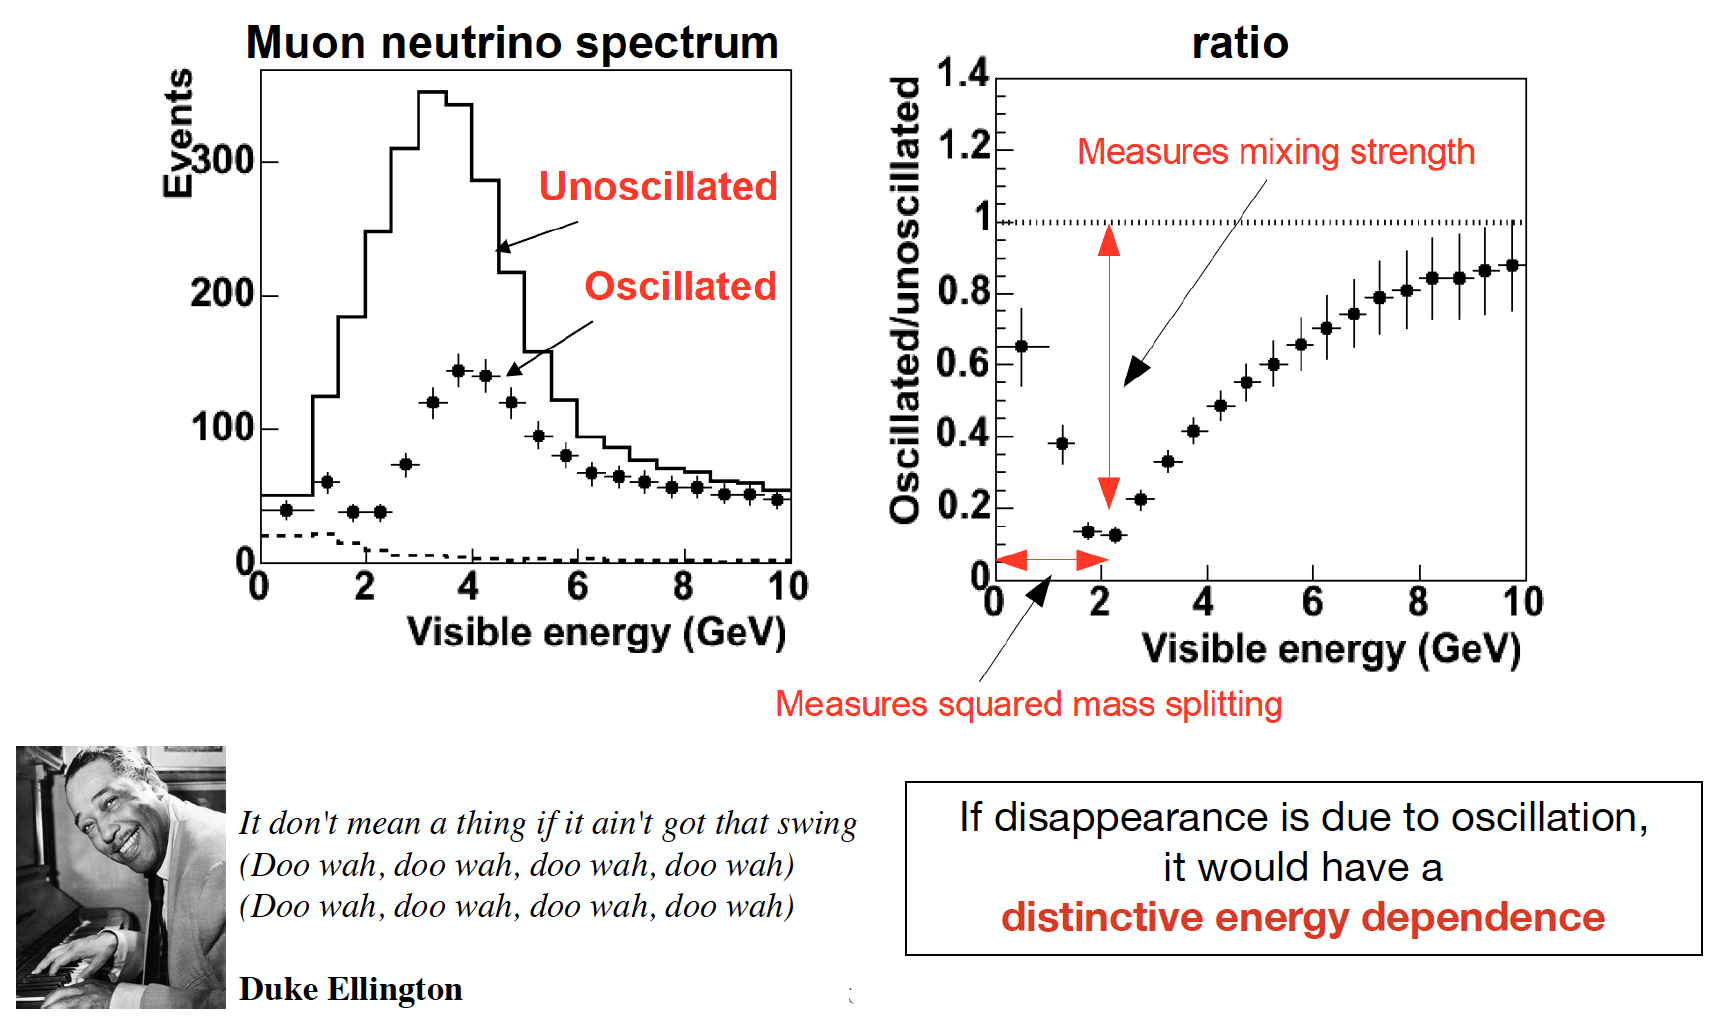
\includegraphics[width=0.95\textwidth]{./images/osc101/disappearance_temp.png}
  \end{center}

\end{frame}

%
%
%

\begin{frame}{Neutrino appearance}

  \begin{center}
    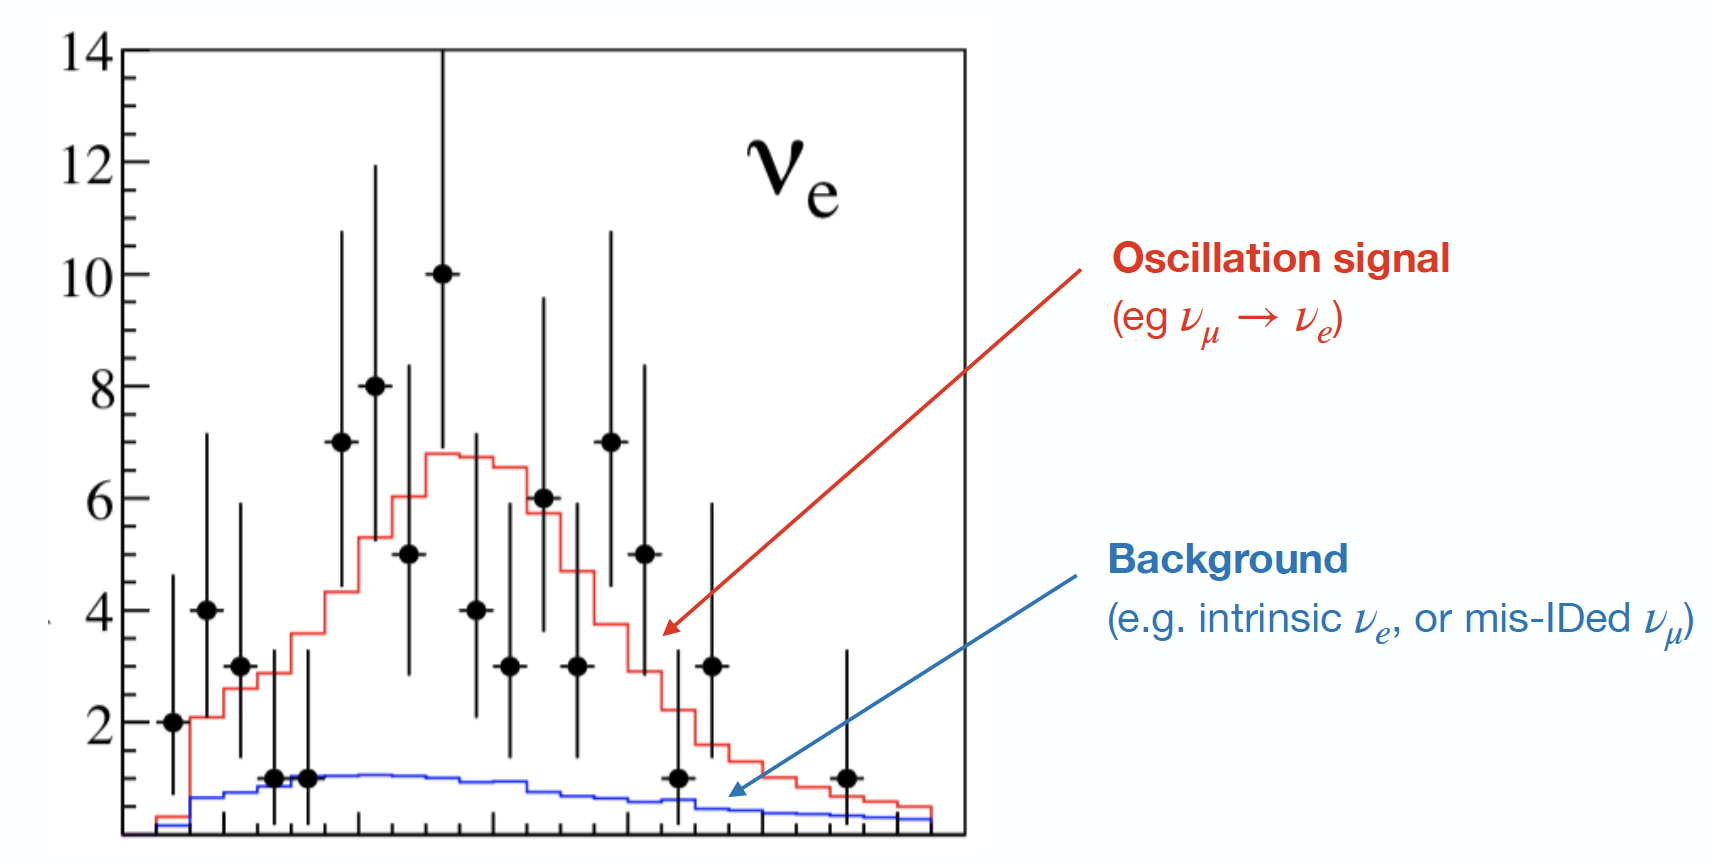
\includegraphics[width=0.95\textwidth]{./images/osc101/appearance_temp.png}
  \end{center}

\end{frame}

%
%
%

\begin{frame}{Representing negative results: The exclusion plot}

Assume you've run a neutrino oscillation experiment, at a particular $L/E$,
and obtained a negative result. How would you represent your result?\\
\vspace{0.3cm}

\begin{columns}
  \begin{column}{0.30\textwidth}
    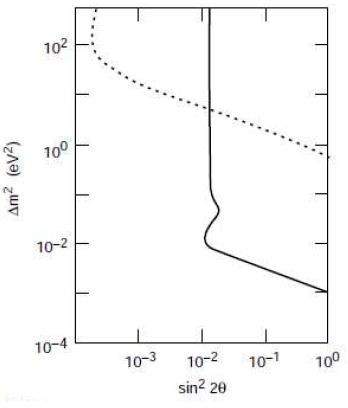
\includegraphics[width=0.99\textwidth]{./images/osc101/exclusion_plot.png}
  \end{column}
  \begin{column}{0.70\textwidth}
     The {\bf exclusion plot}: marks the area of the
     {\color{red}($\theta$, $\Delta m^{2}$)} space that is
     incompatible, at a given statistical significance level, with a
     negative result.\\
     \vspace{0.3cm}
     {\scriptsize
       {\color{capri}
        \underline{Quick check-point}:\\
       }
       \begin{itemize}
       {\color{capri}
        \item Which area is "excluded"?\\
              (On the left or on the right of the line?)
        \item Do you understand the difference between {\bf confidence}
              and a {\bf credible}  interval?
       }
       \end{itemize}
     }
  \end{column}
\end{columns}

\vspace{0.1cm}
The sensitivity to different regions of
the oscillation parameter space
depends on the experimental setup.\\
\vspace{0.3cm}
{\scriptsize
For a negative result, the $\chi^2$ is minimized at the
line corresponding to $sin^2(2\theta)$ = 0.
Typically, the corresponding confidence regions are
constructed using an 1-sided raster scan.\\
}

\end{frame}

%
%
%

\begin{frame}{Representing negative results: The exclusion plot}

Suppose you are studying $\nu_{\alpha} \not\to \nu_{\alpha}$ disappearance,
using a pure $\nu_{\alpha}$ beam.\\
The corresponding survival probability is:\\
\begin{equation*}
     P_{surv} = 1 - P_{\alpha \beta} = 1 - sin^{2} (2\theta) sin^2(\frac{\Delta m^{2}L}{4E})
\end{equation*}
If $N_{\alpha}$ is the number of $\nu_{\alpha}$ events you
would expect to observe, at some distance L, in absence of oscillations, then
the number of events you would expect to observe in the presence of oscillations is
\begin{equation*}
     N^{\prime}_{\alpha} = N_{\alpha} P_{surv}
\end{equation*}
Let $N^{0}_{\alpha}$ be number of events that you would expect to
observe if all produced neutrinos entered your detector. Then
\begin{equation*}
     N_{\alpha} \propto \frac{N^{0}_{\alpha}}{L^2}
\end{equation*}

\end{frame}

%
%
%

\begin{frame}{Representing negative results: The exclusion plot}

Putting everything together,
the number of events you would expect to observe in the presence of oscillations is
\begin{equation*}
     N^{\prime}_{\alpha} \propto \frac{N^{0}_{\alpha}}{L^2}
       \Big\{1 - sin^{2} (2\theta) sin^2(\frac{\Delta m^{2}L}{4E})\Big\}
\end{equation*}

The oscillation {\bf signal} is the observed deficit, which can be written as
\begin{equation*}
     N_{sig} \propto \frac{N^{0}_{\alpha}}{L^2} sin^{2} (2\theta) sin^2(\frac{\Delta m^{2}L}{4E})
\end{equation*}

An appropriate {\bf figure of merit}, a, for the experiment can be formed from
the size of the expected signal relative to the statistical uncertainty on the
background (expected number of events in absence of oscillations):
\begin{equation*}
     a \propto \frac{N_{sig}}{\sqrt{N_{\alpha}}} = \frac{N_{sig}}{\sqrt{N^{0}_{\alpha}}} L
\end{equation*}

\end{frame}

%
%
%

\begin{frame}{Representing negative results: The exclusion plot}

As we wrote earlier, the oscillation signal is given by
\begin{equation*}
     N_{sig} \propto \frac{N^{0}_{\alpha}}{L^2} sin^{2} (2\theta) sin^2(\frac{\Delta m^{2}L}{4E})
\end{equation*}

At low $\Delta m^{2}$, the oscillation signal can be approximated as
\begin{equation*}
     N_{sig} \propto
       \frac{N^{0}_{\alpha}}{L^2}
         sin^{2} (2\theta) \Big(\frac{\Delta m^{2}L}{4E}\Big)^2 \propto
        N^{0}_{\alpha} sin^{2} (2\theta) \Big(\frac{\Delta m^{2}}{E}\Big)^2
\end{equation*}

Therefore
\begin{equation*}
     a \propto \frac{N_{sig}}{\sqrt{N^{0}_{\alpha}}} L =
              \sqrt{N^{0}_{\alpha}} sin^{2} (2\theta) \Big(\frac{\Delta m^{2}}{E}\Big)^2 L
\end{equation*}

The smaller value of $\Delta m^{2}$ that we are sensitive to,
for a given value of a, occurs for $sin^{2} (2\theta)$=1 and it is given by
\begin{equation*}
 {\color{magenta}
  \Delta m^{2} \propto \Big(N^{0}_{\alpha}\Big)^{-1/4} \frac{E}{\sqrt{L}}
 }
\end{equation*}

\end{frame}

%
%
%

\begin{frame}{Representing negative results: The exclusion plot}

The smaller value of $\Delta m^{2}$ that we are sensitive to,
for a given value of a, is
\begin{equation*}
  \Delta m^{2} \propto \Big(N^{0}_{\alpha}\Big)^{-1/4} \frac{E}{\sqrt{L}}
\end{equation*}

Assume that you want to build a new experiment, for the given baseline L,
that can improve the sensitivity to $\Delta m^{2}$ by \underline{one order of magnitude}.
\begin{equation*}
  \Delta m^{2} \rightarrow \Delta m^{2} / 10
\end{equation*}

According to the above, this can be accomplished in one of two ways:
\begin{itemize}
 \item increase the number of events by $10^4$, or
 \item decrease the energy by a factor of 10
\end{itemize}

\end{frame}

%
%
%

\begin{frame}{Representing negative results: The exclusion plot}

Maximum sensitivity to $sin^{2} (2\theta)$ occurs at high $\Delta m^{2}$.
There, the argument of the oscillating term ($sin^2(\frac{\Delta m^{2}L}{4E})$)
is so large that it averages to 1/2.\\

In this case, the expected number of signal events would be
\begin{equation*}
     N_{sig} \propto \frac{N^{0}_{\alpha}}{L^2} sin^{2} (2\theta)
\end{equation*}

and the figure of merit can be written as
\begin{equation*}
     a \propto \frac{N_{sig}}{\sqrt{N^{0}_{\alpha}}} L =
              \sqrt{N^{0}_{\alpha}} sin^{2} (2\theta) \frac{1}{L}
\end{equation*}

The smaller $sin^{2} (2\theta)$ that we are sensitive to,
for a given value of a, is

\begin{equation*}
{\color{magenta}
    sin^{2} (2\theta) \propto \Big( N^{0}_{\alpha} \Big)^{-1/2} L
}
\end{equation*}

Only dependent on $\Big( N^{0}_{\alpha} \Big)^{-1/2}$, so it can be more easily
improved with more data, and independent of E (less sensitive to experimental mistakes).

\end{frame}

%
%
%

\begin{frame}{Representing negative results: The exclusion plot}

\begin{columns}
  \begin{column}{0.25\textwidth}
    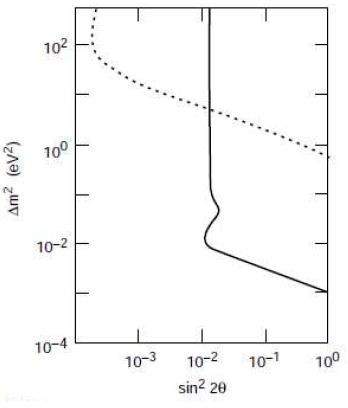
\includegraphics[width=0.90\textwidth]{./images/osc101/exclusion_plot_comments.png}
  \end{column}
  \begin{column}{0.75\textwidth}

    Lowest oscillation parameter values probed
    for a given value of the figure of merit a:

    \begin{equation*}
    {\color{magenta}
      \Delta m^{2} \propto \Big(N^{0}_{\alpha}\Big)^{-1/4} \frac{E}{\sqrt{L}}
    }
    \;\; and \;\;
    {\color{magenta}
      sin^{2} (2\theta) \propto \Big( N^{0}_{\alpha} \Big)^{-1/2} L
    }
    \end{equation*}

  \end{column}
\end{columns}

How about the shape in the middle?
Recall that for low $\Delta m^{2}$
\begin{equation*}
     a \propto \frac{N_{sig}}{\sqrt{N^{0}_{\alpha}}} L =
              \sqrt{N^{0}_{\alpha}} sin^{2} (2\theta) \Big(\frac{\Delta m^{2}}{E}\Big)^2 L
\end{equation*}
Therefore, for a given figure of merit:
{\color{magenta}
    $log\Big( \Delta m^{2} \Big) = a - b \cdot log\Big( sin^{2} (2\theta) \Big)$
}
where a, b are positive constants.\\
\vspace{0.1cm}
In the middle we see the impact of the oscillatory behaviour. The turnover point
between the 2 straight lines occurs roughly at $\Delta m^{2} L / 4E \approx \pi/2$.

\end{frame}

%
%
%

\begin{frame}{Representing positive results: Allowed regions}

{\small
However, if an oscillation signal is measured,
you will want to represent the range of oscillation parameters which are consistent,
to within some level of statistical significance, with
your observed oscillation signal.\\
}

\begin{center}
  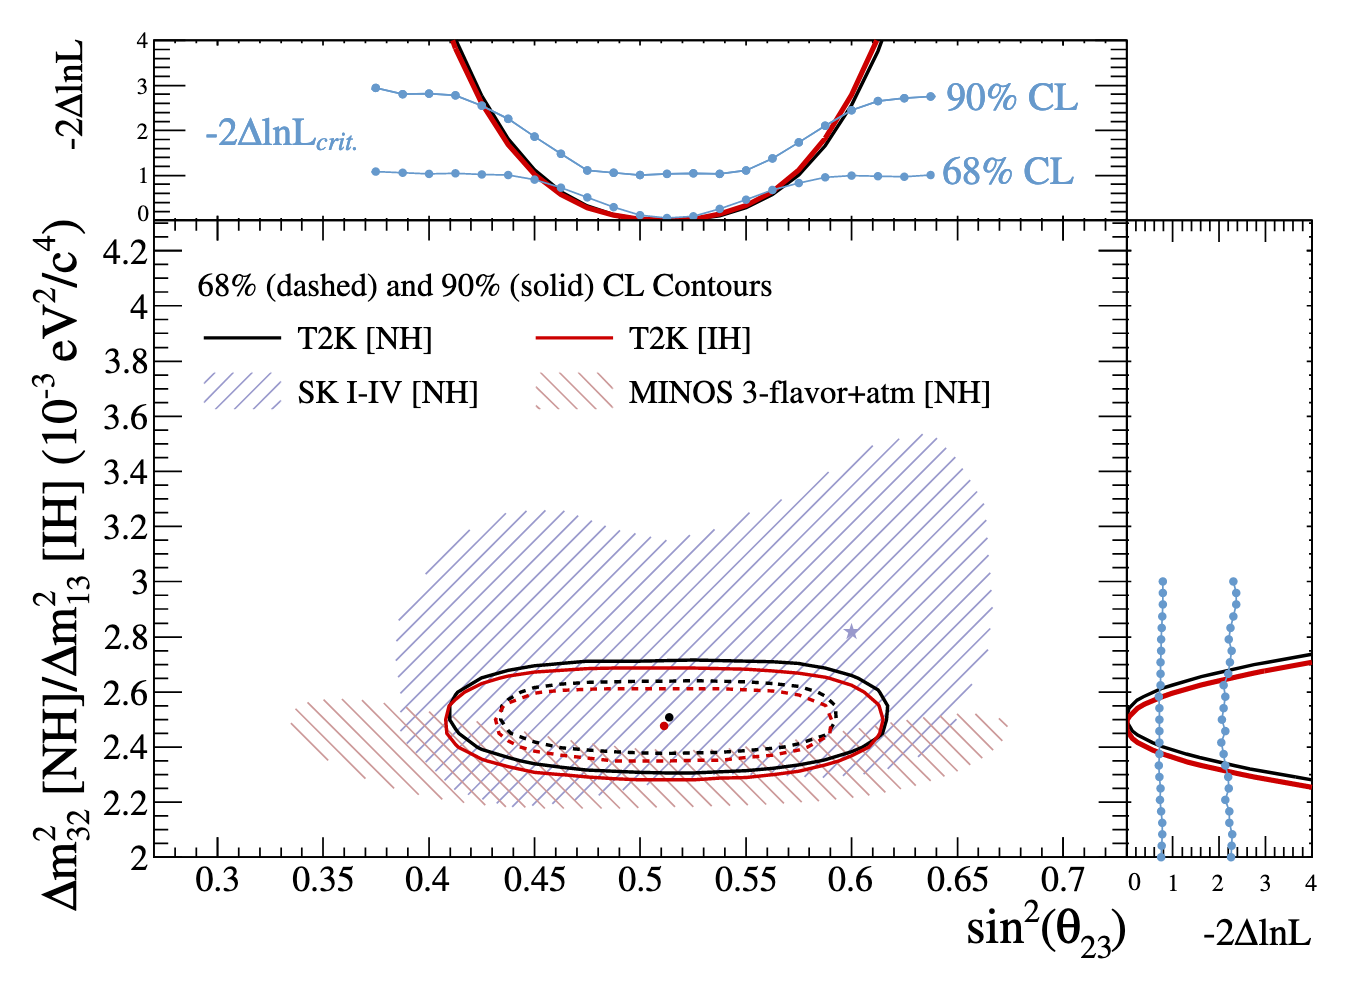
\includegraphics[width=0.67\textwidth]{./images/osc101/allowed_regions.png}\\
  {\tiny \color{blue}[T2K Collaboration, Phys.Rev.Lett. 112 (2014) no.18, 181801]}
\end{center}

\end{frame}

%
%
%

\begin{frame}{Three-flavour case}

The previous picture can be readily generalised for
more neutrino flavours and mass eigenstates:

  \begin{equation}
   \nonumber
   \begin{pmatrix}
    \nu_{e}\\ \nu_{\mu}\\ \nu_{\tau}
   \end{pmatrix}
   =
   \underbrace{
   \begin{pmatrix}
     U_{e1} & U_{e2} & U_{e3} \\
     U_{\mu1} & U_{\mu2} & U_{\mu3} \\
     U_{\tau1} & U_{\tau2} & U_{\tau3} \\
   \end{pmatrix}
   }_\text{$U_{PMNS}$}
   \begin{pmatrix}
    \nu_{1}\\ \nu_{2}\\ \nu_{3}
   \end{pmatrix}
  \end{equation}\\

  Probability for $\nu_{\alpha}\rightarrow\nu_{\beta}$ $(\alpha, \beta: e, \mu, \tau)$ flavour oscillation:

  \begin{eqnarray}
  \nonumber
  \displaystyle
  P_{\alpha\beta} = \delta_{\alpha\beta}
    & - &
      4 {\sum}_{i>j}Re[{\color{red}U_{{\beta}i}U_{{\alpha}i}^{*}U_{{\beta}j}^{*}U_{{\alpha}j}}]
          sin^{2}(\frac{1}{4} \frac{L}{E} {\color{green}{\Delta}m^{2}_{ij}}) \\
    & + &
      2 {\sum}_{i>j}Im[{\color{red}U_{{\beta}i}U_{{\alpha}i}^{*}U_{{\beta}j}^{*}U_{{\alpha}j}}]
          sin(\frac{1}{2} \frac{L}{E} {\color{green}{\Delta}m^{2}_{ij}})
  \nonumber
  \end{eqnarray}

\end{frame}

%
%
%

\begin{frame}{Three-flavour case}

Commonly, the mixing matrix is parameterised as

  \begin{center}
    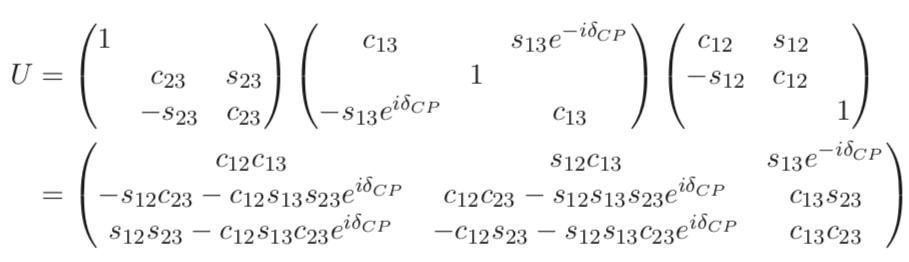
\includegraphics[width=0.88\textwidth]{./images/osc101/pmns_parameterization}\\
  \end{center}

\vspace{0.4cm}
For a purely phenomenological description of neutrino oscillations,
assuming 3 active neutrinos, we need:
\begin{itemize}
\item Any 2 squared mass splittings (e.g. {\color{green}${\Delta}m^{2}_{21}$},{\color{green}${\Delta}m^{2}_{32}$})
\item 3 mixing angles ({\color{red}$\theta_{12}$}, {\color{red}$\theta_{13}$}, {\color{red}$\theta_{23}$})
\item 1 CP invariance violating phase ({\color{red} $\delta_{CP}$})
\end{itemize}

\end{frame}

%
%
%

\begin{frame}{Neutrino oscillations in matter}

Propagation in matter leads to interesting oscillation phenomenology.

\begin{itemize}
\item Ordinary incoherent scattering processes are irrelevant
     \begin{itemize}
        \item Lead to a simple overall decrease of the neutrino beam intensity
        \item Scattering amplitude suppressed by the Fermi constant
      \end{itemize}
\item However, {\color{magenta}
      for {\bf forward scattering}, contributions
      from scattering centres can {\bf add up coherently}}.
      \begin{itemize}
         \item Amplitude still proportional to the Fermi constant,
               but enhanced by the large number of scattering centres.\\
      \end{itemize}
\end{itemize}

\vspace{0.2cm}
Coherent forward scattering possible via
\begin{itemize}
  \item NC interactions with leptons and quarks
  \item CC interactions with quarks
  \item {\color{magenta} \bf CC interactions with leptons}
  \begin{itemize}
    \item Only this type of scattering can lead to flavour-dependent effects
    \item Ordinary matter contains electrons, but no muons or taus
  \end{itemize}
\end{itemize}

\end{frame}


%
% details on matter potential derivation
%

{

\setbeamercolor {frametitle}          {bg=dBG1}
\setbeamercolor {author in head/foot} {bg=dBG1}
\setbeamercolor {title in head/foot}  {bg=dBG2}
\setbeamercolor {date in head/foot}   {bg=dBG3}
\setbeamercolor {date in head/foot}   {fg=dFG3}

\begin{frame}{Matter potential derivation}

For neutrino energies below the masses of the W and Z bosons,
the relevant interaction term in the Langragian is
\begin{equation*}
\mathcal{L}_{CC} = -\frac{G_{F}}{\sqrt{2}}
  \Big( \bar{\ell}_{i} {\gamma}^{\mu} (1-{\gamma}^{5}) U^{\star}_{ij} {\nu}_{j} \Big)
  \Big( \bar{\nu}_{k} U_{\ell k} {\gamma}_{\mu} (1-{\gamma}^{5}) {\ell}_{\ell} \Big)
\end{equation*}

Ordinary matter contains only $e^{-}$, no $\mu^{-}$ or $\tau^{-}$:
\begin{equation*}
\mathcal{L}_{CC} = -\frac{G_{F}}{\sqrt{2}}
  \Big( \bar{e} {\gamma}^{\mu} (1-{\gamma}^{5}) {\nu}_{e} \Big)
  \Big( \bar{\nu}_{e} {\gamma}_{\mu} (1-{\gamma}^{5}) {e} \Big) + h.c.
\end{equation*}

Using the Fierz transform, the above equation becomes:
\begin{equation*}
\mathcal{L}_{CC} = -\frac{G_{F}}{\sqrt{2}}
  \Big( \bar{e} {\gamma}^{\mu} (1-{\gamma}^{5}) e \Big)
  \Big( \bar{\nu}_{e} {\gamma}_{\mu} (1-{\gamma}^{5}) \nu_{e} \Big) + h.c.
\end{equation*}

\end{frame}

%

\begin{frame}{Matter potential derivation}

For unpolarised matter at rest only the $\gamma^0$ term is relevant.\\
The expectation value in the background matter field is
\begin{equation*}
  <\bar{e} \gamma^0 e> = N_e
\end{equation*}
where $N_e$ is the number density of electrons.

% For the electron term,
% the expectation values in the bkg matter field are
% \begin{itemize}
%  \item $<\bar{e} \gamma^0 e> = N_e$,
%  \item $<\bar{e} \vec{\gamma} e> = <\vec{u}_e>$,
%  \item $<\bar{e} \gamma^0 \gamma^5 e> = <\sigma_e \vec{p}_e / E_e>$, and
%  \item $<\bar{e} \vec{\gamma} \gamma^5 e> = <\sigma_e>$,
% \end{itemize}

The corresponding term for neutrinos gives the number of neutrinos.
Therefore, for a single neutrino:

\begin{equation*}
V = -\mathcal{L}_{CC} = \sqrt{2} G_{F} N_{e}
\end{equation*}

\begin{equation*}
V = 7.56 \cdot 10^{-14} \Big( \frac{\rho}{gr/cm^{3}} \Big) \; Y_{e} eV
\end{equation*}
where $Y_{e}$ is the number of electrons per nucleon (in Earth, $Y_{e} \approx 0.5$).

For antineutrinos, V acquires an additional minus sign.

\end{frame}

}


%
%
%

\begin{frame}{Neutrino oscillations in matter}

As we've seen before, for the two-flavour case in vacuum,
neutrino evolution is determined by the Schrodinger equation
\begin{equation}
  i \frac{\partial}{\partial t} \psi = \mathcal{H}_{0} \psi
\end{equation}\\
where $\psi = \Big(\psi_{\alpha}(t), \psi_{\beta}(t)\Big)^T$.
Here, the components $\psi_{\alpha}$ and $\psi_{\beta}$
determine the contribution of each flavour eigenstate
($\alpha$, $\beta$) to $\psi$
\begin{equation}
  \psi = \psi_{\alpha}(t)|\nu_{\alpha}> + \psi_{\beta}(t)|\nu_{\beta}>
\end{equation}\\

The Hamiltonian H is given by
\begin{equation}
   \nonumber
   \mathcal{H}_{0}
   =
   U
   \begin{pmatrix}
     E + \frac{m^2_1}{2E} & 0 \\
     0 & E + \frac{m^2_2}{2E} \\
   \end{pmatrix}
   U^{\dagger}
\end{equation}

In matter:
\begin{equation*}
\mathcal{H}_{0} \rightarrow \mathcal{H} = \mathcal{H}_{0} + \mathcal{V}
\end{equation*}

\end{frame}

%
%
%

\begin{frame}{Neutrino oscillations in matter}

Therefore, for the two-flavor case in matter,
ignoring flavour-independent terms,
the Hamiltonian $\mathcal{H}$ is given by
\begin{equation}
     \nonumber
     \mathcal{H}
     =
     U
     \begin{pmatrix}
       0 & 0 \\
       0 & \frac{\Delta m^2}{2E} \\
     \end{pmatrix}
     U^{\dagger} +
     \begin{pmatrix}
       V & 0 \\
       0 & 0 \\
     \end{pmatrix}
     \Rightarrow
\end{equation}
\begin{equation}
     \nonumber
     \mathcal{H}
     =
     \frac{\Delta m^2}{2E}
     \begin{pmatrix}
       1-cos(2\theta) + 2EV/\Delta m^2  & sin(2\theta) \\
       sin(2\theta)                     & 1 + cos(2\theta) \\
     \end{pmatrix}
\end{equation}

To calculate oscillation probabilities:
\begin{itemize}
\item
{\color{magenta} $\mathcal{H}$ must be diagonalised} -
This would allow us to obtain
  \begin{itemize}
  \item
     the effective energy eigenvalues ($E_{1m}$, $E_{2m}$), and
  \item
     and the effective mixing angle ($\theta_m$).
  \end{itemize}
  \item
  Then $\mathcal{H}$ can be written as $U_m diag(E_{1m},E_{2m}) U_m^{\dagger}$ -
  This is similar to what was done for vacuum but
  \begin{itemize}
  \item
     $\Delta m^{2}/2E$ is replaced by $E_{2m}-E_{1m}$, and
  \item
     $\theta$ is replaced by $\theta_m$.
  \end{itemize}

\end{itemize}

\end{frame}

%
%
%

\begin{frame}{Neutrino oscillations in matter}

For constant V, the effective energy eigenvalues ($E_{1m}$, $E_{2m}$) are given by
\begin{equation}
  \nonumber
  E_{1m} = \frac{V}{2} + \frac{\Delta m^2}{4E}
    \Big\{ 1 - \sqrt{sin^2(2\theta) +
       \Big( cos(2\theta) - \frac{2EV}{\Delta m^2} \Big)^2} \Big\}
\end{equation}

\begin{equation}
  \nonumber
  E_{2m} = \frac{V}{2} + \frac{\Delta m^2}{4E}
    \Big\{ 1 + \sqrt{sin^2(2\theta) +
       \Big( cos(2\theta) - \frac{2EV}{\Delta m^2} \Big)^2} \Big\}
\end{equation}\\

while the effective mixing angle ($\theta_m$) is given by
\begin{equation}
  \nonumber
  sin(2\theta_m) =
    \frac{sin(2\theta)}{\sqrt{sin^2(2\theta) +
       \Big( cos(2\theta) - \frac{2EV}{\Delta m^2} \Big)^2}}
\end{equation}

\begin{equation}
  \nonumber
  cos(2\theta_m) =
    \frac{cos(2\theta)-2EV/\Delta m^2}{\sqrt{sin^2(2\theta) +
       \Big( cos(2\theta) - \frac{2EV}{\Delta m^2} \Big)^2}}
\end{equation}

\end{frame}

%
%
%

\begin{frame}{Neutrino oscillations in matter}

The corresponding oscillation probability in matter is
  \begin{equation}
    \nonumber
    P_{\alpha \beta} = sin^2(2\theta_m) sin^2\Big(
       \frac{\Delta m^2 L}{4E}
       \sqrt{sin^2(2\theta) + \Big( cos(2\theta) - \frac{2EV}{\Delta m^2} \Big)^2}
    \Big)
  \end{equation}

  Let's examine

  \begin{equation}
    \nonumber
    sin(2\theta_m) =
      \frac{sin(2\theta)}{\sqrt{sin^2(2\theta) +
         \Big( cos(2\theta) - \frac{2EV}{\Delta m^2} \Big)^2}}
  \end{equation}

  \begin{itemize}
    \item for low densities ($\rho \rightarrow$ 0), $cos(2\theta) >> \frac{2EV}{\Delta m^2}$:
          {\color{magenta} $sin(2\theta_m) = sin(2\theta)$}
    \item for high densities ($\rho \rightarrow \infty$), $cos(2\theta),sin(2\theta) << \frac{2EV}{\Delta m^2}$:
          {\color{magenta} $sin(2\theta_m) = 0$}
    \item at $cos(2\theta) = \frac{2EV}{\Delta m^2}$:   {\color{magenta} $sin(2\theta_m) = 1$}!!
    \begin{itemize}
      \item Oscillations are {\bf resonantly enhanced}
      \item If $\Delta m^2 > 0$, the resonance occurs for neutrinos while, if
            $\Delta m^2 < 0$ it occurs for antineutrinos.
    \end{itemize}

  \end{itemize}

\end{frame}

%
%
%

\begin{frame}{Neutrino oscillations in matter}

The corresponding oscillation probability in matter is
  \begin{equation}
    \nonumber
    P_{\alpha \beta} = sin^2(2\theta_m) sin^2\Big(
       \frac{\Delta m^2 L}{4E}
       \sqrt{sin^2(2\theta) + \Big( cos(2\theta) - \frac{2EV}{\Delta m^2} \Big)^2}
    \Big)
  \end{equation}

  \begin{center}
    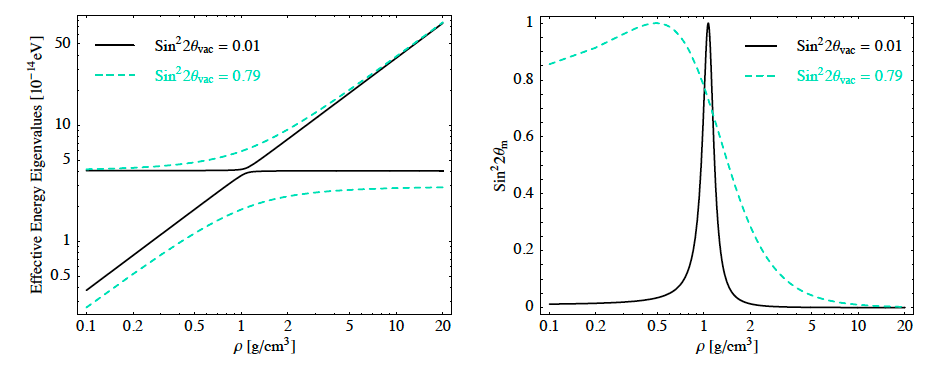
\includegraphics[width=0.88\textwidth]{./images/osc101/MSW1}\\
  \end{center}

\end{frame}

%
%
%

\begin{frame}{Neutrino oscillations in matter}

  in a framework with two flavours we can write
  \begin{equation}
   \nonumber
   \begin{pmatrix}
    \nu_{e}\\ \nu_{\mu}
   \end{pmatrix}
   =
   \begin{pmatrix}
     cos\theta_m & sin\theta_m \\
    -sin\theta_m & cos\theta_m \\
   \end{pmatrix}
   \begin{pmatrix}
    \nu_{1m}\\ \nu_{2m}
   \end{pmatrix}
  \end{equation}

  Therefore
  \begin{equation}
    \nonumber
    |\nu_{e}> = cos\theta_m |\nu_{1m}> + sin\theta_m |\nu_{2m}>
  \end{equation}
  \begin{equation}
    \nonumber
    |\nu_{\mu}> = -sin\theta_m |\nu_{1m}> + cos\theta_m |\nu_{2m}>
  \end{equation}

  Consider the case where, in vacuum, $\theta < \pi/4$.
  \begin{itemize}
    \item in vacuum, $|\nu_{e}>$ is mostly $|\nu_{1}>$
    \item however, if produced near the centre of the Sun, $|\nu_{e}>$ is mostly $|\nu_{2}>$
    \item as it propagates out through slowly decreasing density, it remains in this state
    \item but, in vacuum, $|\nu_{2}>$ is the main component of $|\nu_{\mu}>$
  \end{itemize}
  This is the {\bf MSW (Mikheyev-Smirnov-Wolfenstein) effect}:
  A flavour conversion during an adiabatic transition through an inhomogeneous matter density.
\end{frame}

%
%
%

\begin{frame}{Antineutrino oscillation probabilities}

Change of sign for neutrinos and antineutrinos in the following terms:
\begin{itemize}
  \item Matter potential
  \item $\delta_{CP}$
  \begin{itemize}
    \item $\displaystyle
           \mathcal{L} =
           \frac{g}{\sqrt{2}}
           \bar{e}_{jL} \gamma^{\mu} W^{-}_{\mu} U^{\star}_{jk} \nu_{kL}$ + h.c.
  \end{itemize}
\end{itemize}

\vspace{0.5cm}
In summary:
\begin{equation*}
  \displaystyle
  {\color{magenta}
    P_{\bar{\nu}_{\alpha} \rightarrow \bar{\nu}_{\beta}}(
      {\Delta}m^2_{21}, {\Delta}m^2_{32}, \theta_{12}, \theta_{13}, \theta_{23}, \delta_{CP}, V)
  }
  =
    % P_{\nu_{\alpha} \rightarrow \nu_{\beta}}(
    %    {\Delta}m^2_{21}, {\Delta}m^2_{32}, \theta_{12}, \theta_{13}, \theta_{23}, -\delta_{CP}, -V)
\end{equation*}
\begin{equation*}
  \displaystyle
    P_{\nu_{\alpha} \rightarrow \nu_{\beta}}(
       {\Delta}m^2_{21}, {\Delta}m^2_{32}, \theta_{12}, \theta_{13}, \theta_{23}, -\delta_{CP}, -V)
\end{equation*}

\end{frame}

% %
% %
% %
%
% \begin{frame}{Interdependencies of oscillation channels}
%
% Unitarity implies that:
% \begin{equation*}
% \displaystyle
%   \sum_{\alpha} P_{\nu_{\alpha} \rightarrow \nu_{\beta}} =
%   \sum_{\beta}  P_{\nu_{\alpha} \rightarrow \nu_{\beta}} = 1
% \end{equation*}
%
% 6 conditions, 5 are independent $\rightarrow$
% "23"-rotation commutes with diag(V,0,0)
%
% Reduces the number of independent oscillation probabilities to 2.
%
% Let
% \begin{equation*}
% \displaystyle
%   \tilde{P}_{\nu_{\alpha} \rightarrow \nu_{\beta}} =
%   P_{\nu_{\alpha} \rightarrow \nu_{\beta}} (\theta_{23} \rightarrow \theta_{23} + \frac{\pi}{2})
% \end{equation*}
%
% \end{frame}

%
%
%

\begin{frame}{Interdependencies of oscillation channels}

{\small
  Unitarity
  \begin{equation*}
  \displaystyle
    \sum_{\alpha} P_{\nu_{\alpha} \rightarrow \nu_{\beta}} =
    \sum_{\beta}  P_{\nu_{\alpha} \rightarrow \nu_{\beta}} = 1
  \end{equation*}
  and the fact that the "23" PMNS rotation commutes with
  diag(V,0,0), implies that the are
  {\bf only 2 independent oscillation probabilities}.\\
}

\begin{columns}[T]
 \begin{column}{0.56\textwidth}
   \begin{block}{}
   \begin{itemize}
     \item
      $\displaystyle
      P_{\nu_{e} \rightarrow \nu_{e}} =
        1 -
        {\color{magenta} P_{\nu_{e} \rightarrow \nu_{\mu}} } -
        {\color{magenta} \tilde{P}_{\nu_{e} \rightarrow \nu_{\mu}} }$
      \item
      $\displaystyle
      P_{\nu_{e} \rightarrow \nu_{\tau}} =
        {\color{magenta} \tilde{P}_{\nu_{e} \rightarrow \nu_{\mu}} }$
      \item
      $\displaystyle
      P_{\nu_{\mu} \rightarrow \nu_{e}} =
        {\color{magenta} P_{\nu_{e} \rightarrow \nu_{\mu}} } -
        {\color{blue}    P_{\nu_{\mu} \rightarrow \nu_{\tau}} } +
       {\color{blue}    \tilde{P}_{\nu_{\mu} \rightarrow \nu_{\tau}} }$
      \item
      $\displaystyle
      P_{\nu_{\mu} \rightarrow \nu_{\mu}} =
         1 -
         {\color{magenta} P_{\nu_{e} \rightarrow \nu_{\mu}} } -
         {\color{blue}    \tilde{P}_{\nu_{\mu} \rightarrow \nu_{\tau}} }$
      \item
      $\displaystyle
      P_{\nu_{\tau} \rightarrow \nu_{e}} =
         {\color{magenta} \tilde{P}_{\nu_{e} \rightarrow \nu_{\mu}} } +
         {\color{blue}    P_{\nu_{\mu} \rightarrow \nu_{\tau}} } -
         {\color{blue}    \tilde{P}_{\nu_{\mu} \rightarrow \nu_{\tau}} }$
      \item
      $\displaystyle
      P_{\nu_{\tau} \rightarrow \nu_{\mu}} =
        {\color{blue} \tilde{P}_{\nu_{\mu} \rightarrow \nu_{\tau}} }$
      \item
      $\displaystyle
      P_{\nu_{\tau} \rightarrow \nu_{\tau}} =
        1 -
        {\color{magenta} \tilde{P}_{\nu_{e} \rightarrow \nu_{\mu}} } -
        {\color{blue}    P_{\nu_{\mu} \rightarrow \nu_{\tau}} }$
   \end{itemize}
   \end{block}
 \end{column}
 \begin{column}{0.02\textwidth}
 \end{column}
 \begin{column}{0.42\textwidth}
   \vspace{0.3cm}
   On the left, $\tilde{P}$ is defined as
   \begin{equation*}
   \displaystyle
     \tilde{P}_{\nu_{\alpha} \rightarrow \nu_{\beta}} =
     P_{\nu_{\alpha} \rightarrow \nu_{\beta}} (\theta_{23} \rightarrow \theta_{23} + \frac{\pi}{2})
   \end{equation*}

 \end{column}
\end{columns}

\end{frame}

%
%
%

\begin{frame}{Effect of T, CP and CPT on neutrino oscillation}

\begin{columns}[T]
 \begin{column}{0.45\textwidth}
 \begin{block}{}
 \begin{itemize}
 \item {\bf T symmetry}:
 \begin{equation*}
   \nu_{\alpha} \rightarrow \nu_{\beta}
   \xRightarrow{\;\;\;\;T\;\;\;\;}
   \nu_{\beta} \rightarrow \nu_{\alpha}
 \end{equation*}
 \item {\bf CP symmetry}:
 \begin{equation*}
   \nu_{\alpha} \rightarrow \nu_{\beta}
   \xRightarrow{\;\;\;\;CP\;\;\;}
   \bar{\nu}_{\alpha} \rightarrow \bar{\nu}_{\beta}
 \end{equation*}
 \item {\bf CPT symmetry}:
 \begin{equation*}
   \nu_{\alpha} \rightarrow \nu_{\beta}
   \xRightarrow{\;\;\;CPT\;\;\;}
   \bar{\nu}_{\beta} \rightarrow \bar{\nu}_{\alpha}
 \end{equation*}
 \end{itemize}
 \end{block}
\end{column}
\begin{column}{0.02\textwidth}
\end{column}
\begin{column}{0.53\textwidth}
\vspace{0.3cm}
So, for example, under CPT symmetry:
\begin{equation*}
  P(\nu_{e} \rightarrow \nu_{\mu}) =
  P(\bar{\nu}_{\mu} \rightarrow \bar{\nu}_{e})
\end{equation*}
\begin{equation*}
  P(\nu_{\mu} \rightarrow \nu_{e}) =
  P(\bar{\nu}_{e} \rightarrow \bar{\nu}_{\mu})
\end{equation*}\\
\vspace{0.3cm}
If CP symmetry is violated:
\begin{equation*}
  P(\nu_{\mu} \rightarrow \nu_{e}) \ne
  P(\bar{\nu}_{\mu} \rightarrow \bar{\nu}_{e})
\end{equation*}
\end{column}
\end{columns}

\vspace{0.3cm}

{\color{capri}
\underline{\bf Quick checkpoint:}\\
Why can't we study CP violation via
$\nu_{\mu}$ and $\bar{\nu}_{\mu}$ disappearance?
}

\end{frame}

%
%
%

\begin{frame}{Measuring 3-flavour neutrino oscillations: The big picture}

    \begin{center}
      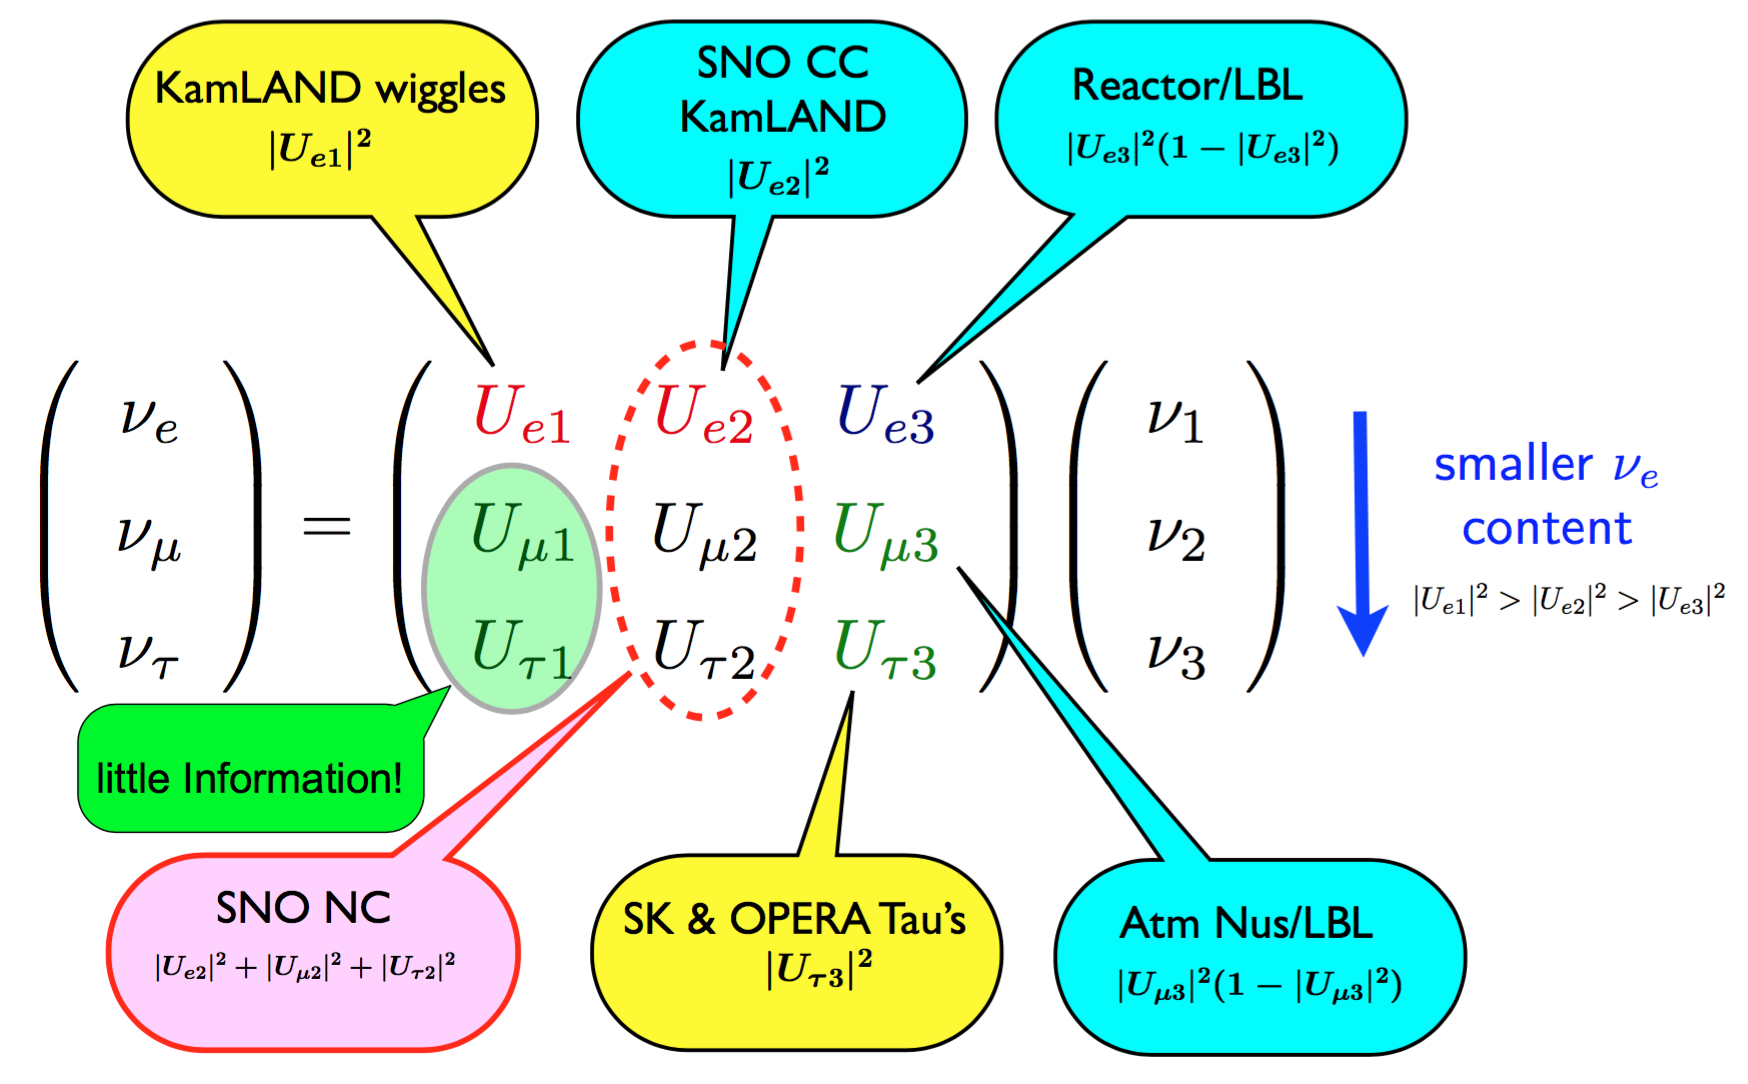
\includegraphics[width=0.88\textwidth]{./images/osc101/upmns_expts_details}\\
    \end{center}

\end{frame}

%
%
%

\begin{frame}{Measuring 3-flavour neutrino oscillations: The big picture}

    \begin{center}
      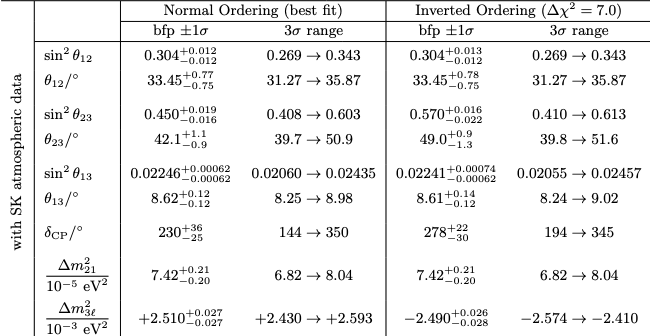
\includegraphics[width=0.88\textwidth]{./images/osc101/nufit_params_v5_1}\\
    \end{center}

    \begin{center}
      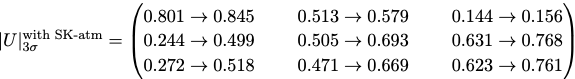
\includegraphics[width=0.70\textwidth]{./images/osc101/nufit_pmns_v5_1}\\
    \end{center}

\end{frame}

%
%
%

\begin{frame}{Measuring 3-flavour neutrino oscillations: 2 $\Delta m^2$ scales}

{\small
 Oscillations have been observed at two squared-mass splitting scales.\\
}
\vspace{0.1cm}

\begin{columns}
  \begin{column}{0.50\textwidth}
    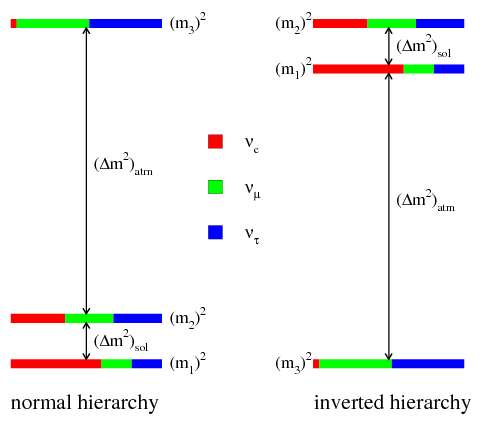
\includegraphics[width=0.85\textwidth]{./images/osc101/mh.png}
  \end{column}
  \begin{column}{0.50\textwidth}
    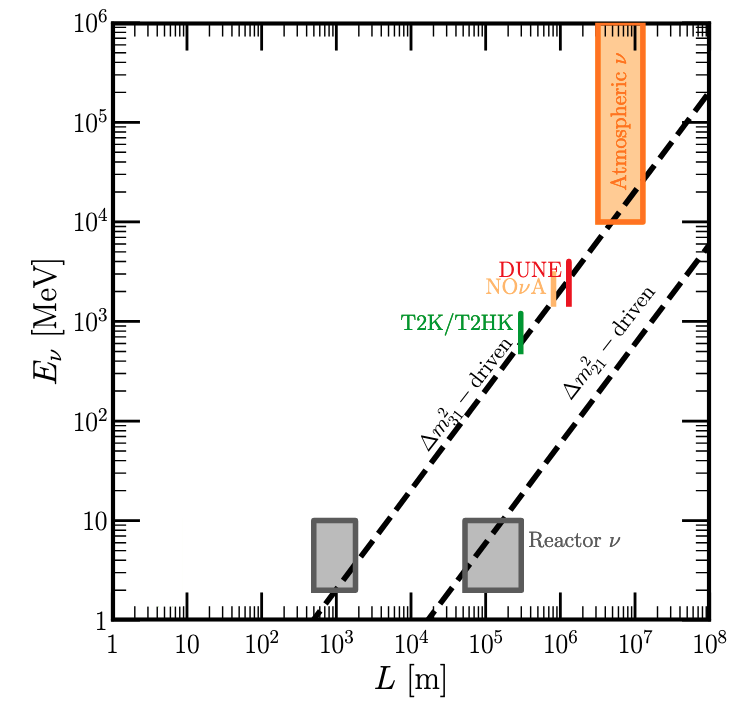
\includegraphics[width=0.80\textwidth]{./images/osc101/expt_L_E_no_sterile}
  \end{column}
\end{columns}

\begin{itemize}
    \item {\color{red} \bf the "solar" splitting}
          {\bf ${\Delta}m^{2}_{21}$ }   $\approx$ 7.5 $\times 10^{-5}$ $eV^{2}/c^{4}$\\
    \vspace{0.1cm}
    \item {\color{red} \bf the "atmospheric" splitting}
          {\bf $|{\Delta}m^{2}_{32}|$ } $\approx$ 2.5 $\times 10^{-3}$ $eV^{2}/c^{4}$\\
\end{itemize}

\vspace{-0.1cm}

\begin{block}{}
{\scriptsize
 Lectures 2-3 we will study the discovery of oscillations
 at each $\Delta m^2$ scale, and lecture 4 will summarise the current status,
 open questions and prospects in the study of 3-flavour oscillations.\\
}
\end{block}

\end{frame}

%
%
%

\begin{frame}{Beyond 3 flavour oscillations}

{\small
  There is a number of {\em anomalous} results that don't fit in the
  3-flavour neutrino oscillation paradigm. If interpreted as oscillations,
  the indicate the existence of sterile neutrinos and a new $\Delta m^2$ scale
  of O(1 eV$^2$). \\
}

  \begin{columns}
    \begin{column}{0.45\textwidth}
      \begin{itemize}
      {\small
        \item {\bf LSND anomaly}\\
           $\sim$50 MeV $\bar{\nu}_{e}$ appearance,\\ $\sim$3.8$\sigma$
        \item {\bf MiniBooNE anomaly}\\
           $\sim$1 GeV $\nu_{e}$ ($\bar{\nu}_{e}$) appearance,\\ $\sim$4.5$\sigma$ ($\sim$2.8$\sigma$)
        \item {\bf Reactor anomaly}\\
           Few-MeV $\bar{\nu}_{e}$ disappearance,\\ $\sim$3.0$\sigma$
        \item {\bf Gallium anomaly}\\
           Sub-MeV $\nu_{e}$ disappearance,\\ $\sim$2.9$\sigma$
      }
      \end{itemize}
    \end{column}
    \begin{column}{0.55\textwidth}
      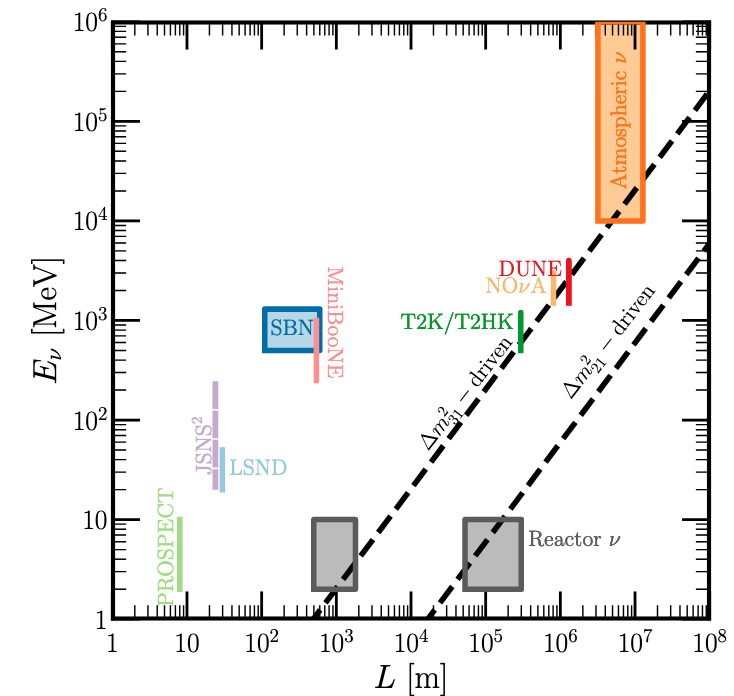
\includegraphics[width=0.90\textwidth]{./images/osc101/expt_L_E}
    \end{column}
  \end{columns}

  \begin{block}{}
  {\scriptsize
   Lecture 5 will summarise anomalous results and tensions in the
   3-flavour oscillation paradigm.\\
  }
  \end{block}

\end{frame}

% %
% %
% %
%
% \begin{frame}{What to read}
%
% \begin{itemize}
% {\scriptsize
% \item
%   PDG review on Neutrino Masses, Mixing, and Oscillations,
%   http://pdg.lbl.gov/2019/reviews/rpp2019-rev-neutrino-mixing.pdf
% \item
%   L. Wolfenstein,
%   Neutrino Oscillations in Matter,
%   Phys.Rev. D17 (1978) 2369-2374
%   {\color{magenta}[Wolfenstein:1977ue]}
% }
% \end{itemize}
%
% \end{frame}
